%! TeX program = lualatex
%! TEX options = -synctex=1 -interaction=nonstopmode -file-line-error --shell-escape "%DOC%"
\documentclass[a4paper,12pt]{article}
\usepackage{luatex85,shellesc}
\usepackage{luainputenc}
\usepackage{graphicx}
\usepackage{amsmath}
\usepackage{amssymb}
\usepackage{amsthm}
\usepackage[libertine]{newtxmath} 
\usepackage[osf]{libertine}
\usepackage{enumerate}
\usepackage{enumitem}
\usepackage[margin=1.6cm]{geometry}
\usepackage[hidelinks]{hyperref}
\usepackage[most]{tcolorbox}
\usepackage{physics}
\usepackage{float}
\usepackage{pgfplots}
\usepackage{wrapfig}
\usepackage{mathtools}
\usepackage[capitalise]{cleveref}
\usepackage{titlesec}
% \usepackage{tikz}
\usepackage{tikz-3dplot}
\usepackage{tensor}
\usepackage{xifthen}
\usepackage{cancel}
\tdplotsetmaincoords{60}{115}
\pgfplotsset{compat=newest}

\usetikzlibrary{calc,backgrounds, decorations.pathmorphing}
\tikzset{snake it/.style={decorate, decoration=snake}}
\newcommand*\circled[1]{\tikz[baseline=(char.base)]{
            \node[shape=circle,draw,inner sep=2pt] (char) {#1};}}

\def\equationautorefname{Eq.}
\newcommand{\bs}[1]{\ensuremath{\boldsymbol{#1}}}
\DeclareMathOperator{\di}{d\!}
\setlength{\jot}{1em}

\renewcommand\thesubsection{\Alph{subsection}}

\newcommand{\mathunderline}[2]{\color{#1}\underline{{\color{black}#2}}\color{black}}

\newcommand{\mytitle}[1]{
	\begin{center}
		\Large \bf
		\textsc{#1}\\
		\vspace{-0.5em}
		\hspace*{0.2\linewidth} \hrulefill \hspace*{0.2\linewidth}
		\vspace{-0.5em}
	\end{center}
}

\newcounter{chapter}

\newcommand{\chapter}[1][]{
	\refstepcounter{chapter}
	\vspace*{-1.5cm}
	\begin{center}
		\Huge \textsc{Assignment}~\ifthenelse{\equal{#1}{}}{\thechapter}{#1}
	\end{center}  
	\vspace{-0.5em}
	\hspace*{0.2\linewidth} \hrulefill \hspace*{0.2\linewidth}
	\vspace{-0.5em}
  }

\newcounter{problem}[chapter]
\newcommand{\problem}{
	\refstepcounter{problem}\par\medskip\section*{Problem~\theproblem}
	}

\newcounter{subproblem}[problem]
\newcommand{\subproblem}{
	\refstepcounter{subproblem}\par\medskip\subsection*{Problem~\theproblem\alph{subproblem}}
	}

%%%%%%%%%%%%%%%%%%%%%%%%%%%%%%%%%%%%%%%%%%%%%%%

\begin{document}

\thispagestyle{empty}

\begin{center}
	\scshape

	\vspace*{2cm}

	\hrule

	\vspace{.7cm}

	{\LARGE{General relativity -- solutions }}

	\vspace{.7cm}

	\hrule

	\vspace{2cm}

	{\large{\textit{Author}:}}\\
	{\large{Michał Siemaszko}}

	\vspace*{2cm}

	\begin{minipage}{0.8\linewidth}
		\begin{flushleft}
			\normalfont
			Those notes were created during course on General relativity in
			summer semester 2019/2020, so during Coronavirus pandemic. We had
			tutorials online and we had to solve problems anyway. Instead of
			solving them on paper and then scanning I decided to improve my
			\LaTeX~skill with \textit{Tikz} package (for plotting). Here is my
			final result.
		\end{flushleft}
	\end{minipage}

	\vspace*{2cm}

	\begin{figure}[H]
		\centering
		\begin{tikzpicture}[domain=0:20]
			\pgfmathsetmacro{\g}{1.5}
			\pgfmathsetmacro{\gg}{1/\g}
			\begin{axis}
				[
					axis lines  = center,
					xlabel={$\tau$},
					ylabel={$a(\tau)$},
					xmin=0,
					xmax=3.5,
					ymin=0,
					ymax=3.5,
					ticks=none
				]

				\addplot[domain = 0:3.14, samples = 1000,color=blue, thick]
				gnuplot {sin(x)};
				\addplot[domain = 0:3.14, samples = 1000,color=red, thick]
				gnuplot {x};
				\addplot[domain = 0:3.14, samples = 1000,color=green, thick]
				gnuplot {sinh(x)};

				\node[inner sep=2pt,text=red] at (2.5,2) {$k=0$};
				\node[inner sep=2pt,text=green] at (.5,1.5) {$k=-1$};
				\node[inner sep=2pt,text=blue] at (1.5,.5) {$k=1$};
			\end{axis}
		\end{tikzpicture}
		% \caption{Radiation dominated universe}
	\end{figure}

	\vfill

	\vspace{1cm}

	{\large{\today}}

	\upshape

\end{center}


\mytitle{ASSIGMENT 1}

\section*{Problem 5}

\begin{wrapfigure}[12]{L}{0.5\linewidth}
    \centering
    \begin{tikzpicture}
        \pgfmathsetmacro{\h}{1.5}
        \pgfmathsetmacro{\ax}{0.5}
        \pgfmathsetmacro{\at}{0}
        \pgfmathsetmacro{\axx}{\ax}
        \pgfmathsetmacro{\att}{\h}
        \pgfmathsetmacro{\bx}{1.5}
        \pgfmathsetmacro{\bt}{0}
        \pgfmathsetmacro{\bxx}{\bx+0.5}
        \pgfmathsetmacro{\btt}{\h}
        \pgfmathsetmacro{\cx}{\ax}
        \pgfmathsetmacro{\ct}{\at}
        \pgfmathsetmacro{\cxx}{\ax + 0.5*\h}
        \pgfmathsetmacro{\ctt}{\at + 0.5*\h}
        \begin{axis}
            [
                axis lines  = center,
                xlabel={$x$},
                ylabel={$t$},
                xmin=-.1,
                xmax=2.5,
                ymin=-.1,
                ymax=2.5,
                xtick={-1},
                xticklabels={$g^{-1}$},
                ytick={-1}
                % ticks=none
            ]
            %
            \coordinate (A) at (axis cs:\ax, \at) {};
            \coordinate (AA) at (axis cs:\axx, \att) {};
            \coordinate (B) at (axis cs:\bx, \bt) {};
            \coordinate (BB) at (axis cs:\bxx, \btt) {};
            \coordinate (C) at (axis cs:\cx, \ct) {};
            \coordinate (CC) at (axis cs:\cxx, \ctt) {};
            %
            \draw[->] (A) -- (AA);
            \draw[->] (B) -- (BB);
            \draw[dotted, ->] (C) -- (CC);
            %
            \node[label={180:{$U^\mu$}},inner sep=2pt] at (AA) {};
            \node[label={0:{$V^\mu$}},inner sep=2pt] at (BB) {};
            \node[label={0:{$P^\mu$}},inner sep=2pt] at (CC) {};
        \end{axis}
    \end{tikzpicture}
    \caption{Setup of experiment}
    % \label{fig:zad1_1}
\end{wrapfigure}

We have given:
%
\begin{align}
    U^\mu & = \left(c,\bs{0}\right)                                       \\
    V^\mu & = \left(\gamma_v c,\gamma_v \bs{v}\right) \label{eq:zad1_vel} \\
    P^\mu & = \left(\frac{h\nu}{c},\bs{p}\right)
\end{align}

We use following relation in this problem:
%
\begin{equation}
    E = -P^\mu V_\mu
\end{equation}
%
This expression is Lorentz invariant and can be calculated in non-moving frame.
So we plug in \autoref{eq:zad1_vel} in this expression to obtain
%
\begin{multline}
    E = -P^\mu V_\mu = \frac{h\nu}{c}\gamma_v c - \gamma_v \bs{v}\bs{p} = 
    \gamma_v\left(h\nu - |\bs{v}||\bs{p}|\cos(\theta)\right) = 
    \left\{|\bs{p}| = \frac{h\nu}{c}\right\} =\\
    \gamma_vh\nu\left(1-\frac{|\bs{v}|}{c}\cos(\theta)\right)
\end{multline}
%
But it is still photon, but with different energy (for moving observer) So
%
\begin{equation}
    \gamma_vh\nu\left(1-\frac{|\bs{v}|}{c}\cos(\theta)\right) = h\nu'
\end{equation}
%
So ratio of those two frequencies is
%
\begin{equation}
    \frac{\nu'}{\nu} = \gamma_v\left(1-\frac{|\bs{v}|}{c}\cos(\theta)\right)
\end{equation}
%
If $\theta = 0$ and $\frac{v}{c} \ll 1 \Rightarrow \gamma_v \simeq 1$ then we
obtain:
%
\begin{equation}
    \boxed{\nu' = \nu \left(1-\frac{v}{c}\right)}
\end{equation}

\newpage

\mytitle{ASSIGMENT 2}

\section*{Problem 1a}

\begin{wrapfigure}[16]{L}{0.5\linewidth}
    \centering
    \begin{tikzpicture}
        \pgfmathsetmacro{\h}{5}
        \pgfmathsetmacro{\w}{5}
        \pgfmathsetmacro{\err}{0.2}
        \pgfmathsetmacro{\ax}{0}
        \pgfmathsetmacro{\ay}{\h}
        \pgfmathsetmacro{\bx}{0}
        \pgfmathsetmacro{\by}{0}
        \pgfmathsetmacro{\cx}{\w}
        \pgfmathsetmacro{\cy}{0}
        \pgfmathsetmacro{\dx}{\w}
        \pgfmathsetmacro{\dy}{\h}

        \coordinate (A) at (\ax, \ay) {};
        \coordinate (B) at (\bx, \by) {};
        \coordinate (C) at (\cx, \cy) {};
        \coordinate (D) at (\dx, \dy) {};
        %
        \draw[->] ($(A)+(0,-\err)$) -- node [text width=1cm, midway,align=left]{h} ($(B)+(0,\err)$);
        \draw[->, dotted] ($(B)+(\err,0)$) -- ($(C)+(-\err,0)$);
        \draw[->, snake it] ($(C)+(0,\err)$) -- ($(D)+(0,-\err)$);
        \draw[->, dotted] ($(D)+(-\err,0)$) -- ($(A)+(\err,0)$);
        %
        \node[label={90:{\circled{1}}}, circle, fill, inner sep=2pt] at (A) {};
        \node[label={270:{\circled{2}}}, circle, fill, inner sep=2pt] at (B) {};
        \node[label={270:{\circled{3}}}, draw, dashed, circle, inner sep=2pt] at (C) {};
        \node[label={90:{\circled{4}}}, draw, dashed, circle, inner sep=2pt] at (D) {};
    \end{tikzpicture}
    \caption{Mass falling in graitational field (1\rightarrow 2), converting to
    photon (2\rightarrow 3), photon traveling up (3\rightarrow 4) and converting
    back to mass (4\rightarrow 1)}
    % \label{fig:zad1_1}
\end{wrapfigure}

Let's take a look at energy changes in above diagram:
\begin{enumerate}[label=\protect\circled{\arabic*}]
    \item $E_1 = mc^2$
    \item $E_2 = mc^2 + mgh$
    \item $E_3 = h\nu = mc^2 + mgh$
    \item $E_4 = h\nu = mc^2 + mgh$
\end{enumerate}
but $E_4 = E_1$ because of energy conservation. It means that photon has to have
different frequency at the height $h$ than it has at the ground. So $E_4 = h\nu'
= mc^2$. From it follows
%
\begin{equation}
    \frac{\nu}{\nu'} = \frac{mc^2+mgh}{mc^2} = 1 + \frac{gh}{c^2}
\end{equation}
%
and it is easy to calculate redshift 
%
\begin{equation}
    \boxed{z = \frac{\nu - \nu'}{\nu'} = \frac{gh}{c^2}}
    \label{eq:prob2a_res}
\end{equation}

\section*{Problem 1b}

\begin{wrapfigure}[16]{R}{0.5\linewidth}
    \centering
    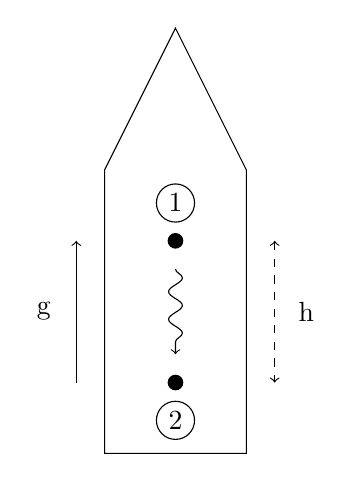
\begin{tikzpicture}[scale=1.8]
        \draw (0,0) -- (0,2) -- (0.5,3) -- (1,2) -- (1, 0) -- cycle;
        \draw[->, snake it] (0.5, 1.3) -- (0.5, 0.7);
        \draw[<->, dashed] (1.2, 1.5) -- node [text width=1cm, midway,align=right]{h}(1.2, 0.5);
        \draw[<-] (-.2, 1.5) -- node [text width=1cm, midway,align=left]{g}(-.2, 0.5);
        %
        \node[label={90:{\circled{1}}}, circle, fill, inner sep=2pt] at (0.5, 1.5) {};
        \node[label={270:{\circled{2}}}, circle, fill, inner sep=2pt] at (0.5, 0.5) {};
    \end{tikzpicture}
    \caption{Two observers in a rocket sending photon}
    % \label{fig:zad1_1}
\end{wrapfigure}

Let's calculate time which light needs to reach observer \circled{2}
%
\begin{equation}
    t = \frac{s}{c} = \frac{h - \frac{gt^2}{2}}{c}
\end{equation}
%
From this expression we get quadratic equation 
%
\begin{equation}
    \frac{g}{2}t^2 + ct - h = 0
\end{equation}
%
for which solution is given by
%
\begin{equation}
    t = \frac{-c + \sqrt{c^2+2gh}}{g}
\end{equation}
%
Velocity of observer \circled{2} after this time is equal 
%
\begin{equation}
    v(t) = \frac{-c + \sqrt{c^2+2gh}}{g} \cdot g = -c + \sqrt{c^2+2gh}
\end{equation}
%
Then redshift formula is given in following way
%
\begin{equation}
    \frac{\nu'}{\nu} = 1 - \frac{v}{c} = 1 - \frac{-c + \sqrt{c^2+2gh}}{c} = 
    2 - \sqrt{1-\frac{2gh}{c^2}} 
\end{equation}
%
We can use Taylor expansion $\sqrt{1-x} = 1-\frac{x}{2}$ we get
%
\begin{equation}
    \boxed{\frac{\nu'}{\nu} = 2 - 1 + \frac{gh}{c^2} = 1 + \frac{gh}{c^2} }
\end{equation}
%
It is exactly the same result as \autoref{eq:prob2a_res}.

\problem

Observer $\mathcal{O}$ is traveling with acceleration $g$ in direction $x_1$. To
calculate his worldline we will use following three conditions
%
\begin{align}
	U^\mu U_\mu & = -1 & U^\mu A_\mu & = 0 & A^\mu A_\mu & = g^2
\end{align}
%
where $U^\mu$ is four-velocity and $A^\mu$ is four-acceleration. First of them
can be obtained by straightforward calculation, second by applying derivative
to first equation i.e.
%
\begin{equation}
	\frac{\dd}{\dd \tau} \left(U^\mu U_\mu\right) = 0 \quad \Rightarrow \quad \left(A^\mu U_\mu\right) = 0
\end{equation}
%
Third is Lorentz invariant and it can be calculated in the moment of launch
namely when $A^\mu=(0,g,0,0)$.

Knowing those three we can write them in explicite form
\begin{align}
	-U_0^2 + \boldsymbol{U}^2    & = -1      &
	\boldsymbol{U}\boldsymbol{A} & = U_0 A_0 &
	-A_0^2 + \boldsymbol{A}^2    & = g^2
\end{align}
%
where bolded letters mean three-vectors.

We square middle equation and plug in left and right equation to obtained
%
\begin{equation}
	(U_0^2 - 1)\boldsymbol{A}^2  = U_0^2  (\boldsymbol{A}^2 -g^2)
\end{equation}
%
Eventually we obtain:
%
\begin{equation}
	\boldsymbol{A}^2 = g^2 U_0^2
\end{equation}
%
and plugin this expression to other equation we also obtain:\footnote{plug it
	into right equation and then use left equation}
%
\begin{equation}
	A_0^2 = g^2 \boldsymbol{U}^2
\end{equation}
%
We can simplify those equation using the fact that this motion is one
dimensional namely $x_2=x_3=0$ and then
%
\begin{align}
	A_1 & = g U_0 & A_0 & = g U_1
\end{align}
%
But $U^\mu = \dot{X^\mu}$ and $A^\mu = \ddot{X^\mu}$ \footnote{dot means
	derivation with respect to proper time}. Substituting
%
\begin{align}
	\ddot{X_1} & = g \dot{X_0} & \ddot{X_0} & = g \dot{X_1}
\end{align}
%
Taking a derivative of left equation and substituting right equation into it we
get
%
\begin{equation}
	\dddot{X_1} = g^2 \dot{X_1}
	\quad \stackrel{\text{after integration}}{\Rightarrow} \quad
	\ddot{X_1} = g^2 X_1
\end{equation}
%
Solution is
%
\begin{equation}
	X_1 = A \sinh(g\tau) + B \cosh(g\tau)
\end{equation}
%
Let's choose initial conditions such as $X_1(0) = g^{-1}$ and $\dot{X_1}=0$. Then
%
\begin{equation}
	X_1 = g^{-1} \cosh(g\tau)
\end{equation}
%
And finally we have
%
\begin{align}
	X_0 & = g^{-1} \sinh(g\tau) & X_1 & = g^{-1} \cosh(g\tau) & X_2 & = 0 & X_3 & = 0
	\label{eq:hiper}
\end{align}
%
\begin{figure}[H]
	\centering
	\begin{tikzpicture}[domain=0:20]
		\pgfmathsetmacro{\g}{1.5}
		\pgfmathsetmacro{\gg}{1/\g}
		\begin{axis}
			[
				axis lines  = center,
				xlabel={$x$},
				ylabel={$t$},
				xmin=0,
				xmax=2.5,
				ymin=0,
				ymax=2.5,
				xtick={\gg},
				xticklabels={$g^{-1}$},
				ytick={-1}
				% ticks=none
			]

			\pgfmathsetmacro{\a}{1.1}
			\pgfmathsetmacro{\ta}{\gg*cosh(\g*\a)}
			\pgfmathsetmacro{\xa}{\gg*sinh(\g*\a)}

			\pgfmathsetmacro{\b}{.1}
			\pgfmathsetmacro{\tb}{\gg*cosh(\g*\b)}
			\pgfmathsetmacro{\xb}{\gg*sinh(\g*\b)}

			\pgfmathsetmacro{\tav}{\gg*cosh(\g*(\a+\b)/2)}
			\pgfmathsetmacro{\xav}{\gg*sinh(\g*(\a+\b)/2)}

			\pgfmathsetmacro{\tp}{\tav*e^(\g*(\a-\b)/2)}
			\pgfmathsetmacro{\xp}{\xav*e^(\g*(\a-\b)/2)}
			%wektory bazowe
			\pgfmathsetmacro{\ezerot}{\ta+cosh(\g*\a)}
			\pgfmathsetmacro{\ezerox}{\xa+sinh(\g*\a)}
			\pgfmathsetmacro{\eonet}{\ta+sinh(\g*\a)}
			\pgfmathsetmacro{\eonex}{\xa+cosh(\g*\a)}

			\coordinate (A) at (axis cs:\ta, \xa) {};
			\coordinate (B) at (axis cs:\tb, \xb) {};
			\coordinate (C) at (axis cs:\tp, \xp) {};
			\coordinate (D) at (axis cs:\tav, \xav) {};
			\coordinate (E) at (axis cs:0,0) {};
			%baza
			\coordinate (ezero) at (axis cs:\ezerot,\ezerox) {};
			\coordinate (eone) at (axis cs:\eonet,\eonex) {};

			\addplot[domain = 0:2.8*\gg, parametric, samples = 1000,color=blue]
			gnuplot {\gg*cosh(\g*t),\gg*sinh(\g*t)};

			% \node[label={180:{$\tau_2$}},circle,fill,inner sep=2pt] at (A) {};
			% \node[label={180:{$\tau_1$}},circle,fill,inner sep=2pt] at (B) {};
			% \node[label={360:{\color{red}$P$}},circle,fill,inner sep=2pt,color=red] at (C) {};
			% \node[label={160:{\color{red}$\frac{\tau_1+\tau_2}{2}$}},circle,fill,inner sep=2pt,color=red] at (D) {};

		\end{axis}
		\begin{scope}[on background layer]
			% \draw[dashed] (A) -- (C);
			% \draw[dashed] (B) -- (C);
			% \draw[dotted,color=red] (C) -- (E);
			%baza
			% \draw[->] (A) -- (ezero);
			% \draw[->] (A) -- (eone);
		\end{scope}
	\end{tikzpicture}
	\caption{Trajectory of $\mathcal{O}$}
	\label{fig:zad1}
\end{figure}

% \bigskip

\problem
%
As a first basis vector we can choose four-velocity namely
%
\begin{equation}
	\boldsymbol{e}_0 = \left(\dot{X_0}, \dot{X_1}, \dot{X_2}, \dot{X_3}\right) =
	\left(\cosh(g\tau), \sinh(g\tau), 0, 0\right)
\end{equation}
%
As a basis vectors in directions $x_2$ and $x_3$ we simply choose
%
\begin{align}
	\boldsymbol{e}_2 = \left(0, 0, 1, 0\right) \\
	\boldsymbol{e}_3 = \left(0, 0, 0, 1\right)
\end{align}
%
And finally we choose vector $\boldsymbol{e}_1$ in a form $\boldsymbol{e}_1 =
	\left(e_1^0, e_1^1, 0, 0\right)$ where $e_1^0$ and $e_1^1$ are chosen in order
to satisfy $\boldsymbol{e}_0 \boldsymbol{e}_1 = 0$ and $(\boldsymbol{e}_0)^2=1$ i.e.
%
\begin{align}
	-e_1^0 \cosh(g\tau) + e_1^1 \sinh(g\tau) & = 0 \\
	-(e_1^0)^2 + (e_1^1)^2 = 1
\end{align}
%
We square first equation and substitute second equation
%
\begin{equation}
	(e_1^0)^2 \cosh^2(g\tau) = (1+(e_1^0)^2) \sinh^2(g\tau)
\end{equation}
%
From this we obtain
%
\begin{align}
	(e_1^0)^2 & = \sinh^2(g\tau) & (e_1^1)^2 & = \cosh^2(g\tau)
\end{align}
%
We can choose positive solution and eventually we get
%
\begin{equation}
	\boldsymbol{e}_1 = \left(\sinh(g\tau), \cosh(g\tau), 0, 0\right)
\end{equation}
%
All vectors
%
\begin{align}
	\boldsymbol{e}_0(\tau) & = \left(\cosh(g\tau), \sinh(g\tau), 0, 0\right) \\
	\boldsymbol{e}_1(\tau) & = \left(\sinh(g\tau), \cosh(g\tau), 0, 0\right) \\
	\boldsymbol{e}_2(\tau) & = \left(0, 0, 1, 0\right)                       \\
	\boldsymbol{e}_3(\tau) & = \left(0, 0, 0, 1\right)
\end{align}
%
Last thing to do is to check whether those are vectors which were obtain without
any rotation. For this I will find a Lorentz boost which transforms initial
basis into this one. Namely consider a boost of time-basis vector

\begin{equation}
	\begin{pmatrix}
		\gamma       & \beta\gamma & 0 & 0 \\
		-\beta\gamma & \gamma      & 0 & 0 \\
		0            & 0           & 1 & 0 \\
		0            & 0           & 0 & 1
	\end{pmatrix}
	\begin{pmatrix}
		1 \\
		0 \\
		0 \\
		0
	\end{pmatrix}
	=
	\begin{pmatrix}
		\gamma       \\
		-\beta\gamma \\
		0            \\
		0
	\end{pmatrix}
\end{equation}
%
So $\gamma$ and $\beta$ have to satisfy:
%
\begin{equation}
	\gamma = \frac{1}{\sqrt{1-v^2}} = \cosh(g\tau) \quad \Rightarrow \quad v = \tanh(g\tau)
\end{equation}
%
Knowing that it is easy to calculate
%
\begin{equation}
	\beta\gamma = \frac{v}{\sqrt{1-v^2}} = \sinh(g\tau)
\end{equation}
%
So indeed we obtain vector $\boldsymbol{e}_0(\tau)$ only via boost (at
$v=\tanh(g\tau)$). The same can be done with vector $\boldsymbol{e}_1(\tau)$

\problem

We define new coordinate system $(\xi_0\equiv\tau, \xi_1, \xi_2, \xi_3)$ where
basis vectors are those defined in problem before. We can write
%
\begin{equation}
	\boldsymbol{x} = \xi^1\boldsymbol{e}_1(\tau) + \xi^2\boldsymbol{e}_2(\tau) +
	\xi^3\boldsymbol{e}_3(\tau) + \boldsymbol{x}_\mathcal{O}(\tau)
\end{equation}
%
where $\boldsymbol{x}_\mathcal{O}(\tau)$ is trajectory of moving frame.

After plugging in all basis vectors explicitly we get
%
\begin{multline}
	\boldsymbol{x} =
	\begin{pmatrix}
		t   \\
		x_1 \\
		x_2 \\
		x_3
	\end{pmatrix}
	=
	\begin{pmatrix}
		\xi^1 \sinh(g\tau) \\
		\xi^1 \cosh(g\tau) \\
		0                  \\
		0
	\end{pmatrix}+
	\begin{pmatrix}
		0     \\
		0     \\
		\xi^2 \\
		0
	\end{pmatrix}+
	\begin{pmatrix}
		0 \\
		0 \\
		0 \\
		\xi^3
	\end{pmatrix}+
	\begin{pmatrix}
		g^{-1}\sinh(g\tau) \\
		g^{-1}\cosh(g\tau) \\
		0                  \\
		0
	\end{pmatrix}= \\
	\begin{pmatrix}
		g^{-1}\sinh(g\tau) + \xi^1 \sinh(g\tau) \\
		g^{-1}\cosh(g\tau) + \xi^1 \cosh(g\tau) \\
		\xi^2                                   \\
		\xi^3
	\end{pmatrix}
	=
	\begin{pmatrix}
		(g^{-1} + \xi^1) \sinh(g\xi^0) \\
		(g^{-1} + \xi^1) \cosh(g\xi^0) \\
		\xi^2                          \\
		\xi^3
	\end{pmatrix}
	\label{eq:motion}
\end{multline}
%
Line element $\dd s^2 = \eta_{\mu\nu} \dd x^\mu \dd x^\nu$ is then equal (we use
chain rule i.e. $\dd x^\mu = \frac{\partial x^\mu}{\partial \xi^\nu}\dd
	\xi^\nu$)
%
\begin{equation}
	\dd s^2 = - \dd t^2 + \dd x_1^2 + \dd x_2^2 + \dd x_3^2
\end{equation}
\begin{align}
	\dd t   & = \frac{\partial t}{\partial \xi^\nu}\dd \xi^\nu =
	(1 + g\xi_1)\cosh(g\xi_0) \dd \xi_0 + \sinh(g\xi_0) \dd \xi_1             \\
	\dd x_1 & = (1 + g\xi_1)\sinh(g\xi_0) \dd \xi_0 + \cosh(g\xi_0) \dd \xi_1 \\
	\dd x_2 & = \dd \xi_2                                                     \\
	\dd x_3 & = \dd \xi_3
\end{align}
After squaring and adding them up we get
%
\begin{align}
	\dd s^2 =  - & (1 + g\xi_1)^2\cosh^2(g\xi_0) \dd \xi_0^2 - \sinh^2(g\xi_0) \dd \xi_1^2 +           \\
	             & (1 + g\xi_1)^2\sinh^2(g\xi_0) \dd \xi_0^2 + \cosh^2(g\xi_0) \dd \xi_1^2 + \nonumber \\
	             & \dd \xi_2^2 +                                                             \nonumber \\
	             & \dd \xi_3^2 \nonumber
\end{align}
After simplification
\begin{equation}
	\boxed{\dd s^2 = -(1+g\xi_1)^2\dd\xi_0^2 + \dd\xi_1^2 + \dd\xi_2^2 + \dd\xi_3^2}
	\label{eq:action}
\end{equation}

\problem

For $\xi^1 \equiv \text{const}$ we can easily derive equation of motion from
\autoref{eq:motion} namely
%
\begin{equation}
	x_1^2 - t^2 = (g^{-1}+\xi^1)^2
\end{equation}
%
which leads to
%
\begin{equation}
	x_1(t) = \sqrt{(g^{-1}+\xi^1)^2 + t^2}
	\label{eq:sqrt}
\end{equation}
%
We take derivative twice
%
\begin{align}
	\dot{x_1}(t)  & = \frac{2t}{2\sqrt{(g^{-1}+\xi^1)^2 + t^2}} \\
	\ddot{x_1}(t) & =
	\frac{\sqrt{(g^{-1}+\xi^1)^2 + t^2} -
		t \frac{2t}{2\sqrt{(g^{-1}+\xi^1)^2 + t^2}}}{(g^{-1}+\xi^1)^2 + t^2} =
	\frac{1}{\sqrt{(g^{-1}+\xi^1)^2 + t^2}} -
	\frac{2t^2}{((g^{-1}+\xi^1)^2 + t^2)^{\frac{3}{2}}}
\end{align}
%
So when $t=0$
%
\begin{equation}
	\boxed{\ddot{x_1}(t)\Big|_{t=0} = \frac{1}{g^{-1}+\xi^1} = \frac{g}{1+g\xi^1}}
\end{equation}


\begin{figure}[H]
	\centering
	\foreach \angle in {0,0.1,0.2}
		{
			\resizebox{0.3\linewidth}{0.3\linewidth}{
				\begin{tikzpicture}[domain=0:5]
					\pgfmathsetmacro{\g}{1.5}
					\pgfmathsetmacro{\gg}{1/\g}
					\pgfmathsetmacro{\xii}{0.5}
					\pgfmathsetmacro{\ggxi}{\gg+\xii}
					\begin{axis}
						[
							axis lines  = center,
							xlabel={$x$},
							ylabel={$t$},
							xmin=-0.1,
							xmax=2.5,
							ymin=-0.1,
							ymax=2.5,
							xtick={\gg,\ggxi},
							xticklabels={$g^{-1}$,$g^{-1}+\xi^1$},
							ytick={-1}
							% ticks=none,
						]

						\pgfmathsetmacro{\g}{1.5}
						\pgfmathsetmacro{\gg}{1/\g}

						\pgfmathsetmacro{\a}{\angle}
						\pgfmathsetmacro{\ta}{\gg*cosh(\g*\a)}
						\pgfmathsetmacro{\xa}{\gg*sinh(\g*\a)}

						\pgfmathsetmacro{\aa}{\angle}
						\pgfmathsetmacro{\taa}{\ggxi*cosh(\g*\aa)}
						\pgfmathsetmacro{\xaa}{\ggxi*sinh(\g*\aa)}

						\pgfmathsetmacro{\b}{.1}
						\pgfmathsetmacro{\tb}{\gg*cosh(\g*\b)}
						\pgfmathsetmacro{\xb}{\gg*sinh(\g*\b)}

						\pgfmathsetmacro{\tav}{\gg*cosh(\g*(\a+\b)/2)}
						\pgfmathsetmacro{\xav}{\gg*sinh(\g*(\a+\b)/2)}

						\pgfmathsetmacro{\tp}{\tav*e^(\g*(\a-\b)/2)}
						\pgfmathsetmacro{\xp}{\xav*e^(\g*(\a-\b)/2)}
						%wektory bazowe
						\pgfmathsetmacro{\ezerot}{\ta+cosh(\g*\a)}
						\pgfmathsetmacro{\ezerox}{\xa+sinh(\g*\a)}
						\pgfmathsetmacro{\eonet}{\ta+sinh(\g*\a)}
						\pgfmathsetmacro{\eonex}{\xa+cosh(\g*\a)}

						\coordinate (A) at (axis cs:\ta, \xa) {};
						\coordinate (AA) at (axis cs:\taa, \xaa) {};
						\coordinate (B) at (axis cs:\tb, \xb) {};
						\coordinate (C) at (axis cs:\tp, \xp) {};
						\coordinate (D) at (axis cs:\tav, \xav) {};
						\coordinate (E) at (axis cs:0,0) {};
						%baza
						\coordinate (ezero) at (axis cs:\ezerot,\ezerox) {};
						\coordinate (eone) at (axis cs:\eonet,\eonex) {};

						% \addplot[domain = 0:1.7, samples=1000, parametric, color=blue]
						% gnuplot {sqrt((\ggxi)^2+t^2),t};	
						\addplot[domain = 0:0.9, parametric, samples = 1000,color=blue]
						gnuplot {\ggxi*cosh(\g*t),\ggxi*sinh(\g*t)};
						\addplot[domain = 0:1.3, parametric, samples = 1000,color=red]
						gnuplot {\gg*cosh(\g*t),\gg*sinh(\g*t)};

						\node[label={180:{${}$}},circle,fill,inner sep=2pt] at (A) {};
						\node[label={180:{${}$}},circle,fill,inner sep=2pt] at (AA) {};
						% \node[label={180:{$\tau_1$}},circle,fill,inner sep=2pt] at (B) {};
						% \node[label={360:{\color{red}$P$}},circle,fill,inner sep=2pt,color=red] at (C) {};
						% \node[label={160:{\color{red}$\frac{\tau_1+\tau_2}{2}$}},circle,fill,inner sep=2pt,color=red] at (D) {};

					\end{axis}
					\begin{scope}[on background layer]
						% \draw[dashed] (A) -- (C);
						% \draw[dashed] (B) -- (C);
						% \draw[dotted,color=red] (C) -- (E);
						%baza
						\draw[->] (A) -- (ezero);
						\draw[->] (A) -- (eone);
						% \draw[dotted] (A)+(3,3) -- (A);
					\end{scope}
				\end{tikzpicture}}
		}
	\caption{\textcolor{red}{Red} line is worldline of \autoref{eq:hiper}
		and \textcolor{blue}{blue} is worldline of \autoref{eq:sqrt}}
	\label{fig:zad4}
\end{figure}

\problem

We start with equation \autoref{eq:action}. We can simplify it and neglect other
spatial dimensions than $\xi^1$ namely
%
\begin{equation}
	\dd s^2 = -(1+g\xi^1)^2 (\dd\xi^0)^2 + (\dd\xi^1)^2
\end{equation}
%
We can change the form to
%
\begin{equation}
	\dd \tau = \dd s = \dd\xi^0 \sqrt{-(1+g\xi^1)^2 + \left(\frac{\dd\xi^1}{\dd\xi^0}\right)^2}
\end{equation}
%
We can now plug in $\xi^1 = \xi^1_\text{em}$ and since emiter does not move in
this frame we can set $\frac{\dd\xi^1}{\dd\xi^0} = 0$:
%
\begin{equation}
	\dd \tau_\text{em} = \dd\xi^0_\text{em} (1+g\xi^1_\text{em})
\end{equation}
%
We can integrate both sides and obtain equation for finite differences
%
\begin{equation}
	\Delta \tau_\text{em} = \Delta \xi^0_\text{em} (1+g\xi^1_\text{em})
\end{equation}
%
We can do similar thing with $\xi^1_\text{rec}$:
%
\begin{equation}
	\Delta \tau_\text{rec} = \Delta \xi^0_\text{rec} (1+g\xi^1_\text{rec})
\end{equation}
%
But left sides of above equations are equal (since line element is invariant
under changing of coordinates) and we can compare them:
%
\begin{equation}
	\frac{\Delta \xi^0_\text{rec}}{\Delta \xi^0_\text{em}} =
	\frac{1+g\xi^1_\text{em}}{1+g\xi^1_\text{rec}} =
	1 + \frac{g\xi^1_\text{em} - g\xi^1_\text{rec}}{1+g\xi^1_\text{rec}} =
	1 - \frac{gh}{1+gh+g\xi^1_\text{em}}
\end{equation}
%
where I put $h = \xi^1_\text{rec} - \xi^1_\text{em}$. After rearranging terms and
substituting $\Delta \xi_\text{rec}^1 = \frac{1}{\nu'}$ and $\Delta
	\xi_\text{em}^1 = \frac{1}{\nu}$
%
\begin{equation}
	\frac{\Delta \xi^0_\text{em} - \Delta \xi^0_\text{rec}}{\Delta \xi^0_\text{em}} =
	\frac{gh}{1+gh+g\xi^1_\text{em}}
\end{equation}
%
\begin{equation}
	\frac{\frac{1}{\nu} - \frac{1}{\nu'}}{\frac{1}{\nu}} =
	\frac{gh}{1+gh+g\xi^1_\text{em}}
	\quad \Rightarrow \quad
	\boxed{z = \frac{\nu' - \nu}{\nu'} = \frac{gh}{1+gh+g\xi^1_\text{em}}}
\end{equation}
%
We can now assume that $g$ is small and using Taylor expansion $\frac{1}{1+x}
	\simeq 1-x$
%
\begin{gather}
	z = gh(1-gh-g\xi^1_\text{em}) = gh - (gh)^2 - g^2h\xi^1_\text{em} \simeq gh \nonumber \\
	z = gh
\end{gather}
%
so the same result as photon in gravitational field.

\mytitle{assigment 3}

\section*{Problem 1}

\begin{equation}
    \mathcal{L}(x^\mu,\dot{x}^\mu) =
    \frac{1}{2}g_{\mu\nu}[x^\mu(\lambda)]\dot{x}^\mu\dot{x}^\nu, \quad
    \dot{x}^{\mu} \equiv \frac{\di x^\mu}{\dd\lambda}
\end{equation}

\begin{multline}
    \delta\int\limits_{\lambda1}^{\lambda2}\mathcal{L}(x^\mu,\dot{x}^\mu)\dd\lambda =
    \int\limits_{\lambda1}^{\lambda2}
    \left(\frac{\partial\mathcal{L}(x^\mu,\dot{x}^\mu)}{\partial x^\sigma}\delta x^\sigma +
    \frac{\partial\mathcal{L}(x^\mu,\dot{x}^\mu)}{\partial \dot{x}^\sigma}\delta \dot{x}^\sigma\right)\dd\lambda = \\
    \int\limits_{\lambda1}^{\lambda2}
    \left(\frac{1}{2}\dot{x}^\mu\dot{x}^\nu \partial_\sigma g_{\mu\nu} \delta x^\sigma +
    \frac{1}{2}g_{\mu\nu}(\delta_{\mu\sigma} \dot{x}^\nu + \delta_{\nu\sigma} \dot{x}^\mu)\delta \dot{x}^\sigma\right)\dd\lambda
\end{multline}
%
Let's take a look at second part of the integral:
%
\begin{multline}
    \frac{1}{2}\int\limits_{\lambda1}^{\lambda2}
    \left\{g_{\mu\nu}(\delta_{\mu\sigma}
    \dot{x}^\nu + \delta_{\nu\sigma} \dot{x}^\mu)\delta \dot{x}^\sigma\right\}\dd\lambda =
    %
    \frac{1}{2}\int\limits_{\lambda1}^{\lambda2}
    \left\{g_{\sigma\nu}\dot{x}^\nu + g_{\mu\sigma}\dot{x}^\mu \right\}
    \delta\dot{x}^\sigma\dd\lambda = \\
    %
    \frac{1}{2}\int\limits_{\lambda1}^{\lambda2}
    \frac{\partial}{\partial\lambda}\left(\left\{
    g_{\sigma\nu}\dot{x}^\nu + g_{\mu\sigma}\dot{x}^\mu
    \right\}\delta x^\sigma\right)\dd\lambda -
    \frac{1}{2}\int\limits_{\lambda1}^{\lambda2}
    \frac{\partial}{\partial\lambda}\left\{
    g_{\sigma\nu}\dot{x}^\nu + g_{\mu\sigma}\dot{x}^\mu
    \right\}\delta x^\sigma\dd\lambda= \\
    %
    \frac{1}{2}\underbrace{\left\{g_{\sigma\nu}\dot{x}^\nu + g_{\mu\sigma}\dot{x}^\mu\right\} \delta x^\sigma \Bigg|_{\lambda1}^{\lambda2}}_{=0} -
    \frac{1}{2}\int\limits_{\lambda1}^{\lambda2}
    \left\{
    \partial_{\mu}g_{\sigma\nu}\dot{x}^\mu\dot{x}^\nu + g_{\sigma\nu}\ddot{x}^\nu +
    \partial_{\nu}g_{\sigma\mu}\dot{x}^\nu\dot{x}^\mu + g_{\sigma\mu}\ddot{x}^\mu
    \right\}\delta x^\sigma\dd\lambda \\
    %
\end{multline}
\begin{equation}
    \delta\int\limits_{\lambda1}^{\lambda2}\mathcal{L}(x^\mu,\dot{x}^\mu)\dd\lambda =
    \frac{1}{2}\int\limits_{\lambda1}^{\lambda2}
    \left(\partial_\sigma g_{\mu\nu}\dot{x}^\mu\dot{x}^\nu -
    \partial_{\mu}g_{\sigma\nu}\dot{x}^\mu\dot{x}^\nu - g_{\sigma\nu}\ddot{x}^\nu -
    \partial_{\nu}g_{\sigma\mu}\dot{x}^\nu\dot{x}^\mu - g_{\sigma\mu}\ddot{x}^\mu\right)\delta x^\sigma \dd\lambda
\end{equation}
%
We want
%
\begin{equation}
    \delta\int\limits_{\lambda1}^{\lambda2}\mathcal{L}(x^\mu,\dot{x}^\mu)\dd\lambda = 0
\end{equation}
%
but since $\delta x^\sigma$ can be arbitrary the rest has to be equal $0$, namely
%
\begin{equation}
    \partial_\sigma g_{\mu\nu}\dot{x}^\mu\dot{x}^\nu -
    \partial_{\mu}g_{\sigma\nu}\dot{x}^\mu\dot{x}^\nu - g_{\sigma\nu}\ddot{x}^\nu -
    \partial_{\nu}g_{\sigma\mu}\dot{x}^\nu\dot{x}^\mu - g_{\sigma\mu}\ddot{x}^\mu = 0
\end{equation}
%
or after rearranging elements
%
\begin{equation}
    \boxed{2 g_{\sigma\mu}\ddot{x}^\mu + \left(\partial_{\nu}g_{\sigma\mu} + 
    \partial_{\mu}g_{\sigma\nu} - \partial_\sigma g_{\mu\nu}\right)\dot{x}^\mu\dot{x}^\nu = 0}
\end{equation}


\mytitle{ASSIGMENT 4}

\section*{Problem 1}

Parallel transport of a vector $V=v^\mu\partial_\mu$ along the curve s
$\gamma:\lambda\mapsto\left[x^1(\lambda),\dots,x^n(\lambda)\right]$:
%
\begin{equation}
    \frac{\dd v^\mu}{\dd\lambda} +
    \Gamma_{\nu\sigma}^{\mu}\left[x(\lambda)\right]v^\nu\frac{\dd x^\sigma}{\dd \lambda}=0
\end{equation}
%
We change coordinates, namely $V = v^\mu\partial_\mu
    = v^\mu\frac{\partial}{\partial x^\mu}=u^\nu\frac{\partial}{\partial y^\nu}$ and
$\gamma:\lambda'\mapsto\left[y^1(\lambda'),\dots,y^n(\lambda')\right]$
%
First we want to obtain transormation rule for vectors namely
%
\begin{equation}
    v^\nu\frac{\partial y^k}{\partial x^\nu}
    = V(y^k) =
    u^\mu\frac{\partial y^k}{\partial y^\mu} = u^k
\end{equation}
%
and for $\Gamma_{\mu\sigma}^\rho=\frac{\partial^2 \xi^\mu}{\partial x^\nu \partial x^\sigma}
    \frac{\partial x^\rho}{\partial\xi^\mu}$
%
\begin{multline}
    \Gamma_{\nu\sigma}'^\rho =
    \frac{\partial}{\partial y^\sigma}
    \left(\frac{\partial \xi^\mu}{\partial y^\nu}\right)
    \frac{\partial y^\rho}{\partial\xi^\mu}=
    \frac{\partial}{\partial y^\sigma}
    \left(\frac{\partial \xi^\mu}{\partial x^\alpha}\frac{\partial x^\alpha}{\partial y^\nu}\right)
    \frac{\partial y^\rho}{\partial x^\beta}\frac{\partial x^\beta}{\partial\xi^\mu}=
    \overbrace{\left[\frac{\partial^2 \xi^\mu}{\partial x^\alpha \partial x^\kappa}
            \frac{\partial x^\alpha}{\partial y^\nu}
            \frac{\partial x^\kappa}{\partial y^\sigma} +
            \frac{\partial \xi^\mu}{\partial x^\alpha}
            \frac{\partial^2 x^\alpha}{\partial y^\nu \partial y^\sigma}\right]}^{
        \frac{\partial^2 \xi^\mu}{\partial y^\nu \partial y^\sigma}~(*)}
    \frac{\partial y^\rho}{\partial x^\beta}\frac{\partial x^\beta}{\partial\xi^\mu}= \\
    \underbrace{\frac{\partial^2 \xi^\mu}{\partial x^\alpha \partial x^\kappa}
        \frac{\partial x^\beta}{\partial\xi^\mu} }_{=\Gamma_{\alpha\kappa}^\beta}
    \frac{\partial x^\kappa}{\partial y^\sigma}
    \frac{\partial x^\alpha}{\partial y^\nu}
    \frac{\partial y^\rho}{\partial x^\beta}
    +
    \frac{\partial^2 x^\alpha}{\partial y^\nu \partial y^\sigma}
    \frac{\partial y^\rho}{\partial x^\beta}
    \underbrace{\frac{\partial \xi^\mu}{\partial x^\alpha}
        \frac{\partial x^\beta}{\partial\xi^\mu}}_{=\delta_\alpha^\beta}=
    \Gamma_{\alpha\kappa}^\beta
    \frac{\partial x^\kappa}{\partial y^\sigma}
    \frac{\partial x^\alpha}{\partial y^\nu}
    \frac{\partial y^\rho}{\partial x^\beta}
    +
    \frac{\partial^2 x^\alpha}{\partial y^\nu \partial y^\sigma}
    \frac{\partial y^\rho}{\partial x^\alpha}
\end{multline}
%
Plugging those things into
%
\begin{equation}
    \frac{\dd u^\mu}{\dd\lambda'} +
    \Gamma_{\nu\sigma}'^{\mu}\left[y(\lambda')\right]u^\nu\frac{\dd y^\sigma}{\dd \lambda'}=0
\end{equation}
%
we obtain
%
\begin{gather}
    \frac{\partial v^\beta}{\partial\lambda}
    \frac{\partial \lambda}{\partial\lambda'}
    \frac{\partial y^\mu}{\partial x^\beta} +
    v^\beta\frac{\partial^2 y^\mu}{\partial x^\beta \partial x^\alpha}
    \frac{\partial x^\alpha}{\partial \lambda}
    \frac{\partial \lambda}{\partial \lambda'} +
    \left\{\Gamma_{\alpha\kappa}^\beta\left[x(\lambda)\right]
    \frac{\partial x^\kappa}{\partial y^\sigma}
    \frac{\partial x^\alpha}{\partial y^\nu}
    \frac{\partial y^\mu}{\partial x^\beta}
    +
    \frac{\partial^2 x^\alpha}{\partial y^\nu \partial y^\sigma}
    \frac{\partial y^\mu}{\partial x^\alpha}\right\}
    v^\eta \frac{\partial y^\nu}{\partial x^\eta}
    \frac{\partial y^\sigma}{\partial \lambda'}=0
\end{gather}
%
Let's take a look at third term of this sum
%
\begin{multline}
    \left\{\Gamma_{\alpha\kappa}^\beta\left[x(\lambda)\right]
    \frac{\partial x^\kappa}{\partial y^\sigma}
    \frac{\partial x^\alpha}{\partial y^\nu}
    \frac{\partial y^\mu}{\partial x^\beta}
    +
    \frac{\partial^2 x^\alpha}{\partial y^\nu \partial y^\sigma}
    \frac{\partial y^\mu}{\partial x^\alpha}\right\}
    v^\eta \frac{\partial y^\nu}{\partial x^\eta}
    \underbrace{\frac{\partial y^\sigma}{\partial x^\tau}
    \frac{\partial x^\tau}{\partial \lambda}
    \frac{\partial \lambda}{\partial \lambda'}}_{\frac{\partial y^\sigma}{\partial \lambda'}}= \\
    v^\eta\Gamma_{\alpha\kappa}^\beta\left[x(\lambda)\right]
    \underbrace{\frac{\partial x^\kappa}{\partial y^\sigma}
        \frac{\partial y^\sigma}{\partial x^\tau}
        \frac{\partial x^\tau}{\partial \lambda}
        \frac{\partial \lambda}{\partial \lambda'}}_{
        =\frac{\partial x^\kappa}{\partial \lambda}\frac{\partial \lambda}{\partial \lambda'}}
    \underbrace{\frac{\partial x^\alpha}{\partial y^\nu}
        \frac{\partial y^\nu}{\partial x^\eta}}_{\delta_\eta^\alpha}
    \frac{\partial y^\mu}{\partial x^\beta}
    +
    v^\eta\underbrace{\frac{\partial^2 x^\alpha}{\partial y^\nu \partial y^\sigma}
        \frac{\partial y^\nu}{\partial x^\eta}
        \frac{\partial y^\sigma}{\partial x^\tau}}_{
        \frac{\partial^2 x^\alpha}{\partial x^\eta \partial x^\tau} -
        \frac{\partial x^\alpha}{\partial y^\nu}
        \frac{\partial^2 y^\nu}{\partial x^\eta \partial x^\tau}~(*)}
    \frac{\partial x^\tau}{\partial \lambda}
    \frac{\partial \lambda}{\partial \lambda'}
    \frac{\partial y^\mu}{\partial x^\alpha}= \\
    \Gamma_{\alpha\kappa}^\beta\left[x(\lambda)\right]v^\alpha
    \frac{\partial x^\kappa}{\partial \lambda}\frac{\partial \lambda}{\partial \lambda'}
    \frac{\partial y^\mu}{\partial x^\beta} -
    v^\eta\frac{\partial^2 y^\nu}{\partial x^\eta \partial x^\tau}
    \underbrace{\frac{\partial x^\alpha}{\partial y^\nu}
        \frac{\partial y^\mu}{\partial x^\alpha}}_{=\delta^\mu_\nu}
    \frac{\partial x^\tau}{\partial \lambda}
    \frac{\partial \lambda}{\partial \lambda'}=
    \Gamma_{\alpha\kappa}^\beta\left[x(\lambda)\right]v^\alpha
    \frac{\partial x^\kappa}{\partial \lambda}\frac{\partial \lambda}{\partial \lambda'}
    \frac{\partial y^\mu}{\partial x^\beta} -
    v^\eta\frac{\partial^2 y^\mu}{\partial x^\eta \partial x^\tau}
    \frac{\partial x^\tau}{\partial \lambda}
    \frac{\partial \lambda}{\partial \lambda'}
\end{multline}
%
So at the end of the day we have
%
\begin{equation}
    \frac{\partial v^\beta}{\partial\lambda}
    \frac{\partial \lambda}{\partial \lambda'}
    \frac{\partial y^\mu}{\partial x^\beta} +
    v^\beta\frac{\partial^2 y^\mu}{\partial x^\beta \partial x^\alpha}
    \frac{\partial x^\alpha}{\partial \lambda}
    \frac{\partial \lambda}{\partial \lambda'}+
    \Gamma_{\alpha\kappa}^\beta\left[x(\lambda)\right]v^\alpha
    \frac{\partial x^\kappa}{\partial \lambda}
    \frac{\partial \lambda}{\partial \lambda'}
    \frac{\partial y^\mu}{\partial x^\beta}-
    v^\eta\frac{\partial^2 y^\mu}{\partial x^\eta \partial x^\tau}
    \frac{\partial x^\tau}{\partial \lambda}
    \frac{\partial \lambda}{\partial \lambda'} = 0
\end{equation}
%
Which simplifies to
%
\begin{equation}
    \left(\frac{\partial v^\beta}{\partial\lambda} +
    \Gamma_{\alpha\kappa}^\beta\left[x(\lambda)\right]v^\alpha
    \frac{\partial x^\kappa}{\partial \lambda}\right)    
    \frac{\partial \lambda}{\partial \lambda'}
    \frac{\partial y^\mu}{\partial x^\beta} = 0
\end{equation}
%
We can divide by $\frac{\partial \lambda}{\partial \lambda'}$
%
\begin{equation}
    \boxed{\left(\frac{\partial v^\beta}{\partial\lambda} +
        \Gamma_{\alpha\kappa}^\beta\left[x(\lambda)\right]v^\alpha
        \frac{\partial x^\kappa}{\partial \lambda}\right)
        \frac{\partial y^\mu}{\partial x^\beta} = 0}
\end{equation}
%
So indeed this equation is coordinate--covariant.

\section*{Problem 2}

Let $\gamma_{\bs{V}}$ denote the geodesic with tangent vector $\bs{V}_p$ at
point $p$. $\{\bs{e}_\mu\}$ is arbitrary basis chosen at the point $p$ and
normal coordinates are defined as $x(q)=(x^1,\dots,x^n) \Leftrightarrow
q=\gamma_{x^\mu \bs{e}_\mu}$ where $p=\gamma(\lambda=0)$, $q=\gamma(\lambda=1)$
and $\{x^i\}_{i=1}^n \in \mathbb{R}$.

First we let $\bs{V}_p=v^\mu \bs{e}_\mu$. But we know, since we consider
geodesic, that $v^\mu = \frac{\dd x^\mu}{\dd \lambda}$.  On the other hand we
can write normal coordinates of point $q$ as $x(q)=(v^1,\dots,v^n)$. So we have
two conditions
%
\begin{equation}
    \frac{\dd x^\mu}{\dd \lambda} \Big|_{\lambda=0} = v^\mu
    \hspace{1cm}
    x^\mu  \Big|_{\lambda=1}= v^\mu
\end{equation}
%
It is easy to solve this 
%
\begin{equation}
    x^\mu\left(\lambda\right) = v^\mu \lambda + x_\mu\left(0\right)
    \label{eq:ass4_geodesic}
\end{equation}
%
\autoref{eq:ass4_geodesic} describes straight line, because it is linear with
respect to $\lambda$ \footnote{or equivalently $\frac{\dd^2 x^i}{\dd
            \lambda^2}=0$}.
%
Substituting this expression into geodesic equation
%
\begin{equation}
    \frac{\dd^2 x^\mu}{\dd \lambda^2} + 
    \Gamma_{\sigma\rho}^\mu\frac{\dd x^\sigma}{\dd \lambda}\frac{\dd x^\rho}{\dd \lambda} = 0
\end{equation}
%
gives
%
\begin{equation}
    \Gamma_{\sigma\rho}^\mu v^\sigma v^\rho = 0
    \label{eq:ass4_gamma}
\end{equation}
%
But \autoref{eq:ass4_gamma} has to be satisfied for arbitrary $v^\sigma$ and
$v^\rho$ which implies
%
\begin{equation}
    \boxed{\Gamma_{\sigma\rho}^\mu = 0}
\end{equation}
%
\section*{Problem 3}

\subsection{\texorpdfstring{$\partial g = 0$}{TEXT}}

We know that metric transforms as follow:
%
\begin{equation}
    g'_{\alpha\beta} = \frac{\partial x^\mu}{\partial x'^\alpha}
    \frac{\partial x^\nu}{\partial x'^\beta} g_{\mu\nu}
\end{equation}
%
Now choosing $x^\mu = x'^\mu - \frac{1}{2} M_{\alpha\beta}^\mu x'^\alpha
    x'^\beta $ will give us
%
\begin{multline}
    g'_{\alpha\beta} = \frac{\partial
        (x'^\mu - \frac{1}{2} M_{\lambda\sigma}^\mu x'^\lambda x'^\sigma)}{\partial x'^\alpha}
    \frac{\partial
        (x'^\nu - \frac{1}{2} M_{\kappa\eta}^\nu x'^\kappa x'^\eta)}{\partial x'^\beta}
    g_{\mu\nu} =\\
    \left(\delta^\mu_\alpha -
    \frac{1}{2} M_{\lambda\sigma}^\mu
    (\delta^\lambda_\alpha x'^\sigma + x'^\lambda \delta^\sigma_\alpha)\right)
    \left(\delta^\nu_\beta -
    \frac{1}{2} M_{\kappa\eta}^\nu
    (\delta^\kappa_\beta x'^\eta + x'^\kappa \delta^\eta_\beta)\right)g_{\mu\nu} = \\
    \left(\delta^\mu_\alpha -
    \frac{1}{2} M_{\alpha\sigma}^\mu x'^\sigma -
    \frac{1}{2} M_{\lambda\alpha}^\mu x'^\lambda\right)
    \left(\delta^\nu_\beta -
    \frac{1}{2} M_{\beta\eta}^\nu x'^\eta -
    \frac{1}{2} M_{\kappa\beta}^\nu x'^\kappa\right)g_{\mu\nu} = \\
    \left(\delta^\mu_\alpha -
    \frac{1}{2}x'^\sigma( M_{\alpha\sigma}^\mu + M_{\sigma\alpha}^\mu)\right)
    \left(\delta^\nu_\beta -
    \frac{1}{2} x'^\eta (M_{\beta\eta}^\nu + M_{\eta\beta}^\nu)\right)g_{\mu\nu}
\end{multline}
%
We take $\tilde{M}_{\beta\eta}^\nu = \frac{1}{2}(M_{\beta\eta}^\nu +
    M_{\eta\beta}^\nu)$ and write (keeping only linear terms in $x$)
%
\begin{equation}
    g'_{\alpha\beta} =
    \left(\delta^\mu_\alpha -
    x'^\sigma \tilde{M}_{\alpha\sigma}^\mu\right)
    \left(\delta^\nu_\beta -
    x'^\eta \tilde{M}_{\beta\eta}^\nu\right)g_{\mu\nu} =
    g_{\alpha\beta} -
    g_{\alpha\nu} x'^\eta \tilde{M}_{\beta\eta}^\nu -
    g_{\mu\beta} x'^\sigma \tilde{M}_{\alpha\sigma}^\mu =
\end{equation}
%
Now we differentiate both sides
%
\begin{multline}
    \partial'_\lambda g'_{\alpha\beta} =
    \partial'_\lambda g_{\alpha\beta} -
    \partial'_\lambda (g_{\alpha\nu} x'^\eta \tilde{M}_{\beta\eta}^\nu) -
    \partial'_\lambda (g_{\mu\beta} x'^\sigma \tilde{M}_{\alpha\sigma}^\mu) = \\
    \partial'_\lambda g_{\alpha\beta} -
    \partial'_\lambda g_{\alpha\nu} x'^\eta \tilde{M}_{\beta\eta}^\nu -
    g_{\alpha\nu} \delta^\eta_\lambda \tilde{M}_{\beta\eta}^\nu -
    \partial'_\lambda g_{\mu\beta} x'^\sigma \tilde{M}_{\alpha\sigma}^\mu -
    g_{\mu\beta} \delta^\sigma_\lambda \tilde{M}_{\alpha\sigma}^\mu
\end{multline}
%
Now we drop linear terms in $x$ (of the form $x\partial g$)
%
\begin{multline}
    \partial'_\lambda g'_{\alpha\beta} =
    \partial'_\lambda g_{\alpha\beta} -
    g_{\alpha\nu} \tilde{M}_{\beta\lambda}^\nu -
    g_{\mu\beta} \tilde{M}_{\alpha\lambda}^\mu=
    \partial_\tau g_{\alpha\beta} \partial'_\lambda x^\tau -
    g_{\alpha\nu} \tilde{M}_{\beta\lambda}^\nu -
    g_{\mu\beta} \tilde{M}_{\alpha\lambda}^\mu=\\
    \partial_\tau g_{\alpha\beta}
    \left(\delta^\tau_\lambda -
    x'^\sigma \tilde{M}_{\lambda\sigma}^\tau\right) -
    g_{\alpha\nu} \tilde{M}_{\beta\lambda}^\nu -
    g_{\mu\beta} \tilde{M}_{\alpha\lambda}^\mu \simeq
    \partial_\lambda g_{\alpha\beta} -
    g_{\alpha\nu} \tilde{M}_{\beta\lambda}^\nu -
    g_{\mu\beta} \tilde{M}_{\alpha\lambda}^\mu
\end{multline}
%
Now let's substitute Chrisroffel symbol in place of $\tilde{M}$ namely

\begin{equation}
    \tilde{M}_{\alpha\beta}^\gamma =
    \frac{1}{2}
    g^{\gamma\sigma}(\partial_\alpha g_{\sigma\beta}+
    \partial_\beta g_{\sigma\alpha}-
    \partial_\sigma g_{\alpha\beta})
\end{equation}
%
We obtain (using $g_{\alpha\beta} = g_{\beta\alpha}$)
%
\begin{multline}
    2\partial'_\lambda g'_{\alpha\beta} =
    2\partial_\lambda g_{\alpha\beta} -
    \underbrace{g_{\alpha\nu}g^{\nu\sigma}}_{=\delta_\alpha^\sigma}
    (\partial_\beta g_{\sigma\lambda}+
    \partial_\lambda g_{\sigma\beta}-
    \partial_\sigma g_{\beta\lambda})-
    \underbrace{g_{\mu\beta}g^{\mu\sigma}}_{=\delta_\beta^\sigma}
    (\partial_\alpha g_{\sigma\lambda}+
    \partial_\lambda g_{\sigma\alpha}-
    \partial_\sigma g_{\alpha\lambda}) = \\
    2\partial_\lambda g_{\alpha\beta} -
    \mathunderline{green}{\partial_\beta g_{\alpha\lambda}}-
    \mathunderline{red}{\partial_\lambda g_{\alpha\beta}}+
    \mathunderline{blue}{\partial_\alpha g_{\beta\lambda}}-
    \mathunderline{blue}{\partial_\alpha g_{\beta\lambda}}-
    \mathunderline{red}{\partial_\lambda g_{\beta\alpha}}+
    \mathunderline{green}{\partial_\beta g_{\alpha\lambda}}=
    2\partial_\lambda g_{\alpha\beta} -
    2\partial_\lambda g_{\alpha\beta} = 0
\end{multline}
%
So eventually
%
\begin{equation}
    \boxed{\partial'_\lambda g'_{\alpha\beta}=0}
\end{equation}

\subsection{\texorpdfstring{$g=\eta$}{TEXT}}

We try following change of coordinates
%
\begin{equation}
    x'^\mu = N_{~~\alpha}^{\mu~~} y^\alpha
\end{equation}
%
In those coordinates metric looks like
%
\begin{equation}
    g''_{\alpha\beta} =
    \frac{\partial x'^\mu}{\partial y^\alpha}
    \frac{\partial x'^\nu}{\partial y^\beta} g'_{\mu\nu} =
    N^{\mu~~}_{~~\alpha} N^{\nu~~}_{~~\beta} g'_{\mu\nu} =
    (N^{-1})^{~~\mu}_{\alpha~~} g'_{\mu\nu} N^{\nu~~}_{~~\beta} =
    (N^{-1} g' N)_{\alpha\beta}
    \label{eq:ass4_eigen}
\end{equation}
%
We can now diagonalize metric $g'$. We can write
%
\begin{equation}
    g' = C~\eta~C^{-1}
\end{equation}
%
where $\eta$ is diagonal and $C$ is a matrix which consists of eigenvectors of
$g'$. If we will choose $N=C$ then \autoref{eq:ass4_eigen} simplifies to
%
\begin{equation}
    \boxed{g''_{\alpha\beta} = \eta_{\alpha\beta}}
\end{equation}

\chapter{}

\problem

\subproblem

We have given metric
%
\begin{equation}
    \bs{g} = \dd\theta \otimes \dd\theta + \sin^2\theta~\dd\phi \otimes \dd\phi
\end{equation}
%
Only non-zero elements are:
%
\begin{equation}
    g_{11} = 1 \hspace{2cm} g_{22} = \sin^2\theta
\end{equation}
%
Also rmeber that $g^{\alpha\beta} = g_{\alpha\beta}^{-1}$ Let's calculate
connection for that metric:
%
\begin{equation}
    \Gamma^\mu_{\nu\sigma} =
    \frac{1}{2} g^{\mu\rho} \left(
    \partial_\nu g_{\rho\sigma} +
    \partial_\sigma g_{\rho\nu} -
    \partial_\rho g_{\nu\sigma}\right)
\end{equation}
%
It is easy to see that
%
\begin{equation}
    \partial_\nu g_{\rho\sigma} =
    \delta_{1\nu}\delta_{2\rho}\delta_{2\sigma}~2\sin\theta\cos\theta
    \label{eq:ass5_only_non_zero}
\end{equation}
%
where $\partial_1 \equiv \partial_\theta$ and $\partial_2 \equiv \partial_\phi$.
Substituting \cref{eq:ass5_only_non_zero} into connection yields
%
\begin{multline}
    \Gamma^\mu_{\nu\sigma} =
    \frac{1}{2} g^{\mu\rho} \left(
    \delta_{1\nu}\delta_{2\rho}\delta_{2\sigma}~2\sin\theta\cos\theta +
    \delta_{1\sigma}\delta_{2\rho}\delta_{2\nu}~2\sin\theta\cos\theta-
    \delta_{1\rho}\delta_{2\nu}\delta_{2\sigma}~2\sin\theta\cos\theta\right) =\\
    \sin\theta\cos\theta\left(
    g^{2\mu} \delta_{1\nu}\delta_{2\sigma} +
    g^{2\mu} \delta_{1\sigma}\delta_{2\nu} -
    g^{1\mu}\delta_{2\nu}\delta_{2\sigma}\right)
\end{multline}
%
The only non--zero coefficients
%
\begin{equation}
    \Gamma^1_{22} = -\sin\theta\cos\theta
    \hspace*{2cm}
    \Gamma^2_{12} = \Gamma^2_{21} = \frac{\cos\theta}{\sin\theta}
    \label{eq:ass5_coeff}
\end{equation}

\subproblem

Geodesic equation is given by
%
\begin{equation}
    \frac{\partial^2 x^\sigma}{\partial \lambda^2} +
    \Gamma^\sigma_{\mu\nu}
    \frac{\partial x^\mu}{\partial \lambda}
    \frac{\partial x^\nu}{\partial \lambda} = 0
\end{equation}
%
Writing explicitly
%
\begin{subequations}
    \begin{align}
        \frac{\partial^2 x^1}{\partial \lambda^2} +
        \Gamma^{1}_{\mu\nu}
        \frac{\partial x^\mu}{\partial \lambda}
        \frac{\partial x^\nu}{\partial \lambda} & = 0 \\
        %
        \frac{\partial^2 x^2}{\partial \lambda^2} +
        \Gamma^{2}_{\mu\nu}
        \frac{\partial x^\mu}{\partial \lambda}
        \frac{\partial x^\nu}{\partial \lambda} & = 0
    \end{align}
\end{subequations}
%
After plugging in \cref{eq:ass5_coeff} we obtain
%
\begin{subequations}
    \begin{align}
        \frac{\partial^2 \theta}{\partial \lambda^2} -
        \sin\theta\cos\theta
        \frac{\partial \phi}{\partial \lambda}
        \frac{\partial \phi}{\partial \lambda} & = 0 \\
        %
        \frac{\partial^2 \phi}{\partial \lambda^2} +
        2\frac{\cos\theta}{\sin\theta}
        \frac{\partial \theta}{\partial \lambda}
        \frac{\partial \phi}{\partial \lambda} & = 0
    \end{align}
\end{subequations}
%
Now we can set $\theta$ and $\phi$ as affine parameters

\subsection*{$\lambda \rightarrow \theta$}

\begin{subequations}
    \begin{align}
        -\sin\theta\cos\theta
        \frac{\partial \phi}{\partial \theta}
        \frac{\partial \phi}{\partial \theta} & = 0 \\
        %
        \frac{\partial^2 \phi}{\partial \theta^2} +
        2\frac{\cos\theta}{\sin\theta}
        \frac{\partial \phi}{\partial \theta} & = 0
    \end{align}
\end{subequations}
%
Solution to this set of equations is trivial namely
%
\begin{equation}
    \frac{\partial \phi}{\partial \theta} = 0
    \quad \Rightarrow \quad
    \phi = \text{const}
\end{equation}
%
It means that longitudinal lines are geodesics in this metric.

\subsection*{$\lambda \rightarrow \phi$}

\begin{subequations}
    \begin{align}
        \frac{\partial^2 \theta}{\partial \phi^2} -
        \sin\theta\cos\theta                  & = 0 \\
        %
        2\frac{\cos\theta}{\sin\theta}
        \frac{\partial \theta}{\partial \phi} & = 0
    \end{align}
\end{subequations}
%
From second equation we have that
%
\begin{equation}
    \frac{\partial \theta}{\partial \phi} = 0
\end{equation}
% 
but it does not solve first equation for every $\theta$. This system of
equations has solutions only when
%
\begin{equation}
    \sin\theta\cos\theta = 0
    \quad \Rightarrow \quad
    \theta = 0 ~\vee~ \theta = \frac{\pi}{2} ~\vee~ \theta = \pi
\end{equation}
%
since $\theta \in \left[0,\pi\right]$. But for $\theta = 0$ or $\theta = \pi$
geodesic line is just one point, because those are poles. Only $\theta =
    \frac{\pi}{2}$ gives non-trivial geodesic. This line is called equator.


\begin{figure}[h]
    \centering
    \begin{tikzpicture}[tdplot_main_coords, scale = 3.5]
        \coordinate (P1) at ({0},{0},{1});
        \coordinate (P2) at ({0},{0},{-1});
        \coordinate (O) at (0,0,0);
        \pgfmathsetmacro{\rvec}{1.4}
        \pgfmathsetmacro{\thetavec}{45}
        \pgfmathsetmacro{\phivec}{60}

        \tdplotsetcoord{P}{\rvec}{\thetavec}{\phivec}

        \shade[ball color = lightgray, opacity = 0.5] (0,0,0) circle (1cm);

        \tdplotsetrotatedcoords{0}{0}{0};
        \draw[dashed, tdplot_rotated_coords, red] (0,0,0) circle (1);

        \tdplotsetrotatedcoords{-90}{90}{0};
        \draw[dashed, tdplot_rotated_coords, blue] (1,0,0) arc (0:180:1);

        \tdplotsetrotatedcoords{0}{90}{0};
        \draw[dashed, tdplot_rotated_coords, blue] (1,0,0) arc (0:180:1);

        \draw[dashed, gray] (0,0,0) -- (-1,0,0);
        \draw[dashed, gray] (0,0,0) -- (0,-1,0);

        \draw[-stealth] (0,0,0) -- (1.80,0,0) node[below left] {$x$};
        \draw[-stealth] (0,0,0) -- (0,1.30,0) node[below right] {$y$};
        \draw[-stealth] (0,0,0) -- (0,0,1.30) node[above] {$z$};
        \node[right] at (P1) {$P_1$};
        \node[right] at (P2) {$P_2$};

        \draw[-stealth, color=black] (O) -- (P) node[midway,below] {};

        \tdplotdrawarc{(O)}{0.2}{0}{\phivec}{anchor=north}{$\phi$}
        \draw[dashed, color=magenta] (O) -- (Pxy);
        \draw[dashed, color=magenta] (P) -- (Pxy);

        \tdplotsetthetaplanecoords{\phivec}
        \tdplotdrawarc[tdplot_rotated_coords]{(0,0,0)}{0.5}{\thetavec}{0}{anchor=south west}{$\theta$}

        \draw[fill = lightgray!50] (P1) circle (0.5pt);
        \draw[fill = lightgray!50] (P2) circle (0.5pt);
    \end{tikzpicture}
    \caption{Visualization of geodesics -- \textcolor{red}{red} line is equator,
        \textcolor{blue}{blue} lines are two possible meridians, $P_1$ and $P_2$ are poles.}
\end{figure}

\subproblem

\subsection*{$\theta = \frac{\pi}{2},~\phi = 0 \rightarrow \theta = 0,~ \phi = 0$}

We use equation of parallel transport of vector \bs{v} along curve $\gamma$ with
$\frac{\dd \gamma^\mu}{\dd \lambda} = w^\mu$
%
\begin{equation}
    \nabla_{\bs{w}} \bs{v} = 0
\end{equation}
%
We can write it explicitly
%
\begin{equation}
    w^\nu \partial_\nu v^\mu + w^\nu \Gamma^\mu_{\nu\sigma} v^\sigma = 0
\end{equation}
%
or substituting connections I've calculated before
%
\begin{subequations}
    \begin{align}
        w^1 \partial_1 v^1 + w^2 \partial_2 v^1 + w^2 \Gamma^1_{22} v^2                         & = 0 \\
        w^1 \partial_1 v^2 + w^2 \partial_2 v^2 + w^1 \Gamma^2_{12} v^2 + w^2 \Gamma^2_{21} v^1 & = 0
    \end{align}
\end{subequations}
%
If we move along meridian then we can take $\lambda \rightarrow \theta$. From
this we get coefficients $w$ namely $w^1 = \frac{\dd \theta}{\dd \theta} = 1$
and $w^2 = \frac{\dd \phi}{\dd \theta} = 0$. Putting this and connection
coefficients into equations we obtain
%
\begin{subequations}
    \begin{align}
        \partial_1 v^1                                     & = 0 \\
        \partial_1 v^2 + \frac{\cos\theta}{\sin\theta} v^2 & = 0
    \end{align}
\end{subequations}
%
Second equation we multiply by $\sin\theta$ and simplify
%
\begin{subequations}
    \begin{align}
        \partial_1 v^1                        & = 0 \\
        \partial_1 \left(v^2\sin\theta\right) & = 0
    \end{align}
\end{subequations}
%
This gives use
%
\begin{subequations}
    \begin{align}
        v^1 & = C_1                    \\
        v^2 & = \frac{C_2}{\sin\theta}
    \end{align}
\end{subequations}
%
Constants $C_1$ and $C_2$ depends on the vector we transport:
\begin{itemize}
    \item for $\frac{\partial}{\partial \theta}$ we have at the beginning
          ($\theta = \frac{\pi}{2}$) $v=(1,0)$ so $C_1 = 1$ and $C_2 = 0$ so the
          transport
          \begin{equation}
              \bs{v} = (1,0) \rightarrow (1,0) = \bs{v}'
          \end{equation}
          does not change this vector.
    \item for $\frac{\partial}{\partial \phi}$ we have at the beginning
          $v=(0,1)$ so $C_1 = 0$ and $C_2 = 1$ so the transport
          \begin{equation}
              \bs{v} = (0,1) \rightarrow (0,\frac{1}{\sin\theta}) = \bs{v}'
          \end{equation}
          is undefined at point $\theta = 0$
\end{itemize}

\subsection*{$\theta = \frac{\pi}{2},~\phi = 0 \rightarrow \theta = \frac{\pi}{2},~ \phi = \frac{\pi}{4}$}

%
If we move along equator then we can take $\lambda \rightarrow \phi$. From
this we get coefficients $w$ namely $w^1 = \frac{\dd \theta}{\dd \phi} = 0$
and $w^2 = \frac{\dd \phi}{\dd \phi} = 1$. Putting this and connection
coefficients into equations we obtain
%
\begin{subequations}
    \begin{align}
        \partial_2 v^1 - \sin\theta\cos\theta v^2          & = 0 \\
        \partial_2 v^2 + \frac{\cos\theta}{\sin\theta} v^1 & = 0
    \end{align}
\end{subequations}
%
which simplifies to
%
\begin{subequations}
    \begin{align}
        \partial_2 v^1 & = 0 \\
        \partial_2 v^2 & = 0
    \end{align}
\end{subequations}
%
because $\cos\theta \Big|_{\theta=\frac{\pi}{2}}= 0$
%
\begin{subequations}
    \begin{align}
        v^1 & = C_1 \\
        v^2 & = C_2
    \end{align}
\end{subequations}
%
Constants $C_1$ and $C_2$ depends on the vector we transport:
\begin{itemize}
    \item for $\frac{\partial}{\partial \theta}$ we have at the beginning
          ($\phi = 0$) $v=(1,0)$ so $C_1 = 1$ and $C_2 = 0$ so the
          transport
          \begin{equation}
              \bs{v} = (1,0) \rightarrow (1,0) = \bs{v}'
          \end{equation}
          does not change this vector.
    \item for $\frac{\partial}{\partial \phi}$ we have at the beginning
          $v=(0,1)$ so $C_1 = 0$ and $C_2 = 1$ so the transport
          \begin{equation}
              \bs{v} = (0,1) \rightarrow (0,1) = \bs{v}'
          \end{equation}
          does not change this vector.
\end{itemize}

\begin{figure}[h]
    \centering
    \begin{tikzpicture}[tdplot_main_coords, scale = 2.5]
        \coordinate (O) at (0,0,0);

        \pgfmathsetmacro{\rvec}{1}
        \pgfmathsetmacro{\thetavec}{45}
        \pgfmathsetmacro{\phivec}{45}

        \pgfmathsetmacro{\sinphi}{sin(\phivec)}
        \pgfmathsetmacro{\cosphi}{cos(\phivec)}

        \pgfmathsetmacro{\sintheta}{sin(\thetavec)}
        \pgfmathsetmacro{\costheta}{cos(\thetavec)}

        \tdplotsetcoord{P}{\rvec}{\thetavec}{\phivec}

        \shade[ball color = lightgray, opacity = 0.5] (0,0,0) circle (1cm);

        \tdplotsetrotatedcoords{0}{0}{0};
        \draw[dashed, tdplot_rotated_coords, gray] (0,0,0) circle (1);

        \tdplotsetrotatedcoords{-90}{90}{0};
        \draw[dashed, tdplot_rotated_coords, gray] (1,0,0) arc (0:180:1);

        \tdplotsetrotatedcoords{0}{90}{0};
        \draw[dashed, tdplot_rotated_coords, gray] (1,0,0) arc (0:180:1);

        \draw[dashed, gray] (0,0,0) -- (-1,0,0);
        \draw[dashed, gray] (0,0,0) -- (0,-1,0);

        \draw[-stealth] (0,0,0) -- (1.80,0,0) node[below left] {$x$};
        \draw[-stealth] (0,0,0) -- (0,1.30,0) node[below right] {$y$};
        \draw[-stealth] (0,0,0) -- (0,0,1.30) node[above] {$z$};

        \draw[-stealth, color=red]
        (\sinphi,\cosphi,0) -- (\sinphi-\cosphi, \cosphi+\sinphi, 0) node[above]
        {$\frac{\partial}{\partial \phi}$};
        \draw[-stealth, color=red]
        (\sinphi,\cosphi,0) -- (\sinphi,\cosphi,-1) node[left]
        {$\frac{\partial}{\partial \theta}$};

        \draw[-stealth, color=blue]
        (\sintheta,0,\costheta) -- (\sintheta+\costheta,0,\costheta-\sintheta) node[left]
        {$\frac{\partial}{\partial \theta}$};
        \draw[-stealth, color=blue]
        (\sintheta,0,\costheta) -- (\sintheta,1,\costheta) node[above]
        {$\frac{\partial}{\partial \phi}$};

    \end{tikzpicture}
    \caption{Visualization of parallel transport -- \textcolor{red}{red} is
        transport along equator, \textcolor{blue}{blue} is transport along
        meridians.}
\end{figure}

\problem

Materic is given by
%
\begin{equation}
    g_{\nu\mu} =
    \begin{pmatrix}
        -B(r) & 0    & 0   & 0               \\
        0     & A(r) & 0   & 0               \\
        0     & 0    & r^2 & 0               \\
        0     & 0    & 0   & r^2\sin^2\theta
    \end{pmatrix}
\end{equation}
%
We can calculate connection coefficients using relation
%
\begin{equation}
    \Gamma^\mu_{\nu\sigma} =
    \frac{1}{2} g^{\mu\rho} \left(
    \partial_\nu g_{\rho\sigma} +
    \partial_\sigma g_{\rho\nu} -
    \partial_\rho g_{\nu\sigma}\right)
\end{equation}
%
Becasue metric is diagonal we can simplify this expression:
%
\begin{equation}
    \Gamma^\mu_{\nu\sigma} =
    \frac{1}{2} g^{\mu\mu} \left(
    \partial_\nu g_{\mu\sigma} +
    \partial_\sigma g_{\mu\nu} -
    \partial_\mu g_{\nu\sigma}\right)
\end{equation}
%
\begin{subequations}
    \begin{align}
        \Gamma^0 & =
        -\frac{1}{2} \frac{1}{B(r)}
        \begin{pmatrix}
            0       & \dot{B} & 0 & 0 \\
            \dot{B} & 0       & 0 & 0 \\
            0       & 0       & 0 & 0 \\
            0       & 0       & 0 & 0 \\
        \end{pmatrix} \\
        \Gamma^1 & =
        \frac{1}{2} \frac{1}{A(r)}
        \begin{pmatrix}
            \dot{B} & 0       & 0   & 0               \\
            0        & \dot{A} & 0   & 0               \\
            0        & 0       & -2r & 0               \\
            0        & 0       & 0   & -2r\sin^2\theta \\
        \end{pmatrix} \\
        \Gamma^2 & =
        \frac{1}{2} \frac{1}{r^2}
        \begin{pmatrix}
            0 & 0  & 0  & 0                         \\
            0 & 0  & 2r & 0                         \\
            0 & 2r & 0  & 0                         \\
            0 & 0  & 0  & -r^22\sin\theta\cos\theta \\
        \end{pmatrix} =
        \begin{pmatrix}
            0 & 0           & 0           & 0                     \\
            0 & 0           & \frac{1}{r} & 0                     \\
            0 & \frac{1}{r} & 0           & 0                     \\
            0 & 0           & 0           & -\sin\theta\cos\theta \\
        \end{pmatrix} \\
        \Gamma^3 & =
        \frac{1}{2} \frac{1}{r^2\sin^2\theta}
        \begin{pmatrix}
            0 & 0              & 0                        & 0                        \\
            0 & 0              & 0                        & 2r\sin^2\theta           \\
            0 & 0              & 0                        & r^22\sin\theta\cos\theta \\
            0 & 2r\sin^2\theta & r^22\sin\theta\cos\theta & 0                        \\
        \end{pmatrix} =
        \begin{pmatrix}
            0 & 0           & 0                             & 0                             \\
            0 & 0           & 0                             & \frac{1}{r}                   \\
            0 & 0           & 0                             & \frac{\cos\theta}{\sin\theta} \\
            0 & \frac{1}{r} & \frac{\cos\theta}{\sin\theta} & 0                             \\
        \end{pmatrix}
    \end{align}
\end{subequations}
%
Geodesic equation
%
\begin{equation}
    \frac{\partial^2 x^\sigma}{\partial \lambda^2} +
    \Gamma^\sigma_{\mu\nu}\frac{\partial x^\mu}{\partial \lambda}\frac{\partial x^\nu}{\partial \lambda} = 0
\end{equation}
%
\subsection*{$\sigma = 0$}

\begin{equation}
    \frac{\partial^2 t}{\partial \lambda^2} -
    \frac{1}{2} \frac{1}{B(t)}
    \begin{pmatrix}
        \frac{\partial t}{\partial \lambda}      &
        \frac{\partial r}{\partial \lambda}      &
        \frac{\partial \theta}{\partial \lambda} &
        \frac{\partial \phi}{\partial \lambda}
    \end{pmatrix}
    \begin{pmatrix}
        0       & \dot{B} & 0 & 0 \\
        \dot{B} & 0       & 0 & 0 \\
        0       & 0       & 0 & 0 \\
        0       & 0       & 0 & 0 \\
    \end{pmatrix}
    \begin{pmatrix}
        \frac{\partial t}{\partial \lambda}      \\[6pt]
        \frac{\partial r}{\partial \lambda}      \\[6pt]
        \frac{\partial \theta}{\partial \lambda} \\[6pt]
        \frac{\partial \phi}{\partial \lambda}
    \end{pmatrix} = 0
\end{equation}

\begin{equation}
    \frac{\partial^2 t}{\partial \lambda^2} -
    \frac{1}{2} \frac{1}{B(t)}
    \left(-2\dot{B} \frac{\partial t}{\partial \lambda}\frac{\partial r}{\partial \lambda}\right) = 0
\end{equation}

\begin{equation}
    \frac{\partial^2 t}{\partial \lambda^2} +
    \frac{\dot{B}}{B}
    \frac{\partial t}{\partial \lambda}\frac{\partial r}{\partial \lambda} = 0
\end{equation}

\subsection*{$\sigma = 1$}

\begin{equation}
    \frac{\partial^2 r}{\partial \lambda^2} +
    \frac{1}{2} \frac{1}{A(r)}
    \begin{pmatrix}
        \frac{\partial t}{\partial \lambda}      &
        \frac{\partial r}{\partial \lambda}      &
        \frac{\partial \theta}{\partial \lambda} &
        \frac{\partial \phi}{\partial \lambda}
    \end{pmatrix}
    \begin{pmatrix}
        \dot{B} & 0       & 0   & 0               \\
        0        & \dot{A} & 0   & 0               \\
        0        & 0       & -2r & 0               \\
        0        & 0       & 0   & -2r\sin^2\theta \\
    \end{pmatrix}
    \begin{pmatrix}
        \frac{\partial t}{\partial \lambda}      \\[6pt]
        \frac{\partial r}{\partial \lambda}      \\[6pt]
        \frac{\partial \theta}{\partial \lambda} \\[6pt]
        \frac{\partial \phi}{\partial \lambda}
    \end{pmatrix} = 0
\end{equation}

\begin{equation}
    \frac{\partial^2 r}{\partial \lambda^2} +
    \frac{\dot{B}}{2A}\left(\frac{\partial t}{\partial \lambda}\right)^2 +
    \frac{\dot{A}}{2A}\left(\frac{\partial r}{\partial \lambda}\right)^2 -
    \frac{r}{A}\left(\frac{\partial \theta}{\partial \lambda}\right)^2 -
    \frac{r\sin^2\theta}{A}\left(\frac{\partial \phi}{\partial \lambda}\right)^2 = 0
\end{equation}

\subsection*{$\sigma = 2$}

\begin{equation}
    \frac{\partial^2 \theta}{\partial \lambda^2} +
    \begin{pmatrix}
        \frac{\partial t}{\partial \lambda}      &
        \frac{\partial r}{\partial \lambda}      &
        \frac{\partial \theta}{\partial \lambda} &
        \frac{\partial \phi}{\partial \lambda}
    \end{pmatrix}
    \begin{pmatrix}
        0 & 0           & 0           & 0                     \\
        0 & 0           & \frac{1}{r} & 0                     \\
        0 & \frac{1}{r} & 0           & 0                     \\
        0 & 0           & 0           & -\sin\theta\cos\theta \\
    \end{pmatrix}
    \begin{pmatrix}
        \frac{\partial t}{\partial \lambda}      \\[6pt]
        \frac{\partial r}{\partial \lambda}      \\[6pt]
        \frac{\partial \theta}{\partial \lambda} \\[6pt]
        \frac{\partial \phi}{\partial \lambda}
    \end{pmatrix} = 0
\end{equation}

\begin{equation}
    \frac{\partial^2 \theta}{\partial \lambda^2} +
    \frac{2}{r} \frac{\partial r}{\partial \lambda}\frac{\partial \theta}{\partial \lambda} -
    \sin\theta\cos\theta \left(\frac{\partial \phi}{\partial \lambda}\right)^2 = 0
\end{equation}

\subsection*{$\sigma = 2$}

\begin{equation}
    \frac{\partial^2 \phi}{\partial \lambda^2} +
    \begin{pmatrix}
        \frac{\partial t}{\partial \lambda}      &
        \frac{\partial r}{\partial \lambda}      &
        \frac{\partial \theta}{\partial \lambda} &
        \frac{\partial \phi}{\partial \lambda}
    \end{pmatrix}
    \begin{pmatrix}
        0 & 0           & 0                             & 0                             \\
        0 & 0           & 0                             & \frac{1}{r}                   \\
        0 & 0           & 0                             & \frac{\cos\theta}{\sin\theta} \\
        0 & \frac{1}{r} & \frac{\cos\theta}{\sin\theta} & 0                             \\
    \end{pmatrix}
    \begin{pmatrix}
        \frac{\partial t}{\partial \lambda}      \\[6pt]
        \frac{\partial r}{\partial \lambda}      \\[6pt]
        \frac{\partial \theta}{\partial \lambda} \\[6pt]
        \frac{\partial \phi}{\partial \lambda}
    \end{pmatrix} = 0
\end{equation}

\begin{equation}
    \frac{\partial^2 \phi}{\partial \lambda^2} +
    \frac{2}{r} \frac{\partial r}{\partial \lambda}\frac{\partial \phi}{\partial \lambda} +
    2\frac{\cos\theta}{\sin\theta} \frac{\partial \theta}{\partial \lambda}\frac{\partial \phi}{\partial \lambda} = 0
\end{equation}
%
Gathering all equations
%

\begin{subequations}
    \begin{align}
        0 & = \frac{\partial^2 t}{\partial \lambda^2} +
        \frac{\dot{B}}{B}
        \frac{\partial t}{\partial \lambda}\frac{\partial r}{\partial \lambda}       \\
        %
        0 & = \frac{\partial^2 r}{\partial \lambda^2} +
        \frac{\dot{B}}{2A}\left(\frac{\partial t}{\partial \lambda}\right)^2 +
        \frac{\dot{A}}{2A}\left(\frac{\partial r}{\partial \lambda}\right)^2 -
        \frac{r}{A}\left(\frac{\partial \theta}{\partial \lambda}\right)^2 -
        \frac{r\sin^2\theta}{A}\left(\frac{\partial \phi}{\partial \lambda}\right)^2 \\
        %
        0 & = \frac{\partial^2 \theta}{\partial \lambda^2} +
        \frac{2}{r} \frac{\partial r}{\partial \lambda}\frac{\partial \theta}{\partial \lambda} -
        \sin\theta\cos\theta \left(\frac{\partial \phi}{\partial \lambda}\right)^2   \\
        %
        0 & = \frac{\partial^2 \phi}{\partial \lambda^2} +
        \frac{2}{r} \frac{\partial r}{\partial \lambda}\frac{\partial \phi}{\partial \lambda} +
        2\frac{\cos\theta}{\sin\theta} \frac{\partial \theta}{\partial \lambda}\frac{\partial \phi}{\partial \lambda}
    \end{align}
\end{subequations}

\problem

Metric is given by
%
\begin{equation}
    \bs{g} = - c^2 \left(1−2\frac{GM}{rc^2}\right) \dd t \otimes \dd t  + \dd \bs{x} \otimes \dd \bs{x}
\end{equation}
%
We can calculate infinitesimal interval of two events in this metric
%
\begin{equation}
    \dd s^2 = - c^2 \left(1−2\frac{GM}{rc^2}\right) \dd t^2 + \dd \bs{x}^2
\end{equation}
%
Simplifying this and assuming that the person has not been moving for whole year
we can write
%
\begin{equation}
    \dd s^2 = \dd t^2 \left(- c^2 \left(1−2\frac{GM}{rc^2}\right)  +
    \frac{\dd \bs{x}^2}{\dd t^2}\right) =
    - \dd t^2c^2 \left(1−2\frac{GM}{rc^2}\right)
\end{equation}
%
We can now calculate the proper time
%
\begin{equation}
    c^2 \dd \tau^2 = \dd t^2c^2 \left(1−2\frac{GM}{rc^2}\right)
    \quad \Rightarrow \quad
    \dd \tau = \dd t \sqrt{1−2\frac{GM}{rc^2}}
\end{equation}
%
and finite version
%
\begin{equation}
    \Delta \tau = \Delta t \sqrt{1−2\frac{GM}{rc^2}}
\end{equation}
%
Now I take $\Delta \tau_{0}$ to be proper time of person's feet and
$\Delta \tau_{H}$ for head (in distance $H$ from feet). Now I can calculate the
difference
%
\begin{equation}
    \Delta \tau_{H} - \Delta \tau_{0} =
    \Delta t \left(\sqrt{1−2\frac{GM}{(r+H)c^2}} - \sqrt{1−2\frac{GM}{rc^2}}\right)
\end{equation}
%
Because expressions under square are small I can Taylor expand them (using
$\sqrt{1-2x} \simeq 1 -x$)
%
\begin{equation}
    \Delta \tau_{H} - \Delta \tau_{0} =
    \Delta t \left(-\frac{GM}{(r+H)c^2} + \frac{GM}{rc^2} \right) =
    \Delta t \frac{GM}{c^2} \left(\frac{1}{r} - \frac{1}{r+H}\right) =
    \Delta t \frac{GM}{c^2r} \frac{H}{r+H}
\end{equation}
%
Plugging all the constants and assuming that person has height 1.8 m
after 1 year time difference is
%
\begin{equation}
    \Delta \tau_{H} - \Delta \tau_{0} = 6.3 \times 10^{-9}~\text{s}
\end{equation}

\begin{figure}[H]
    \centering
    \begin{tikzpicture}[domain=0:2]
        \pgfmathsetmacro{\C}{6.96e-1}
        \pgfmathsetmacro{\R}{6371000}
        \pgfmathsetmacro{\dt}{31557600}
        \begin{axis}
            [
            axis lines  = left,
            xlabel={$x$~[m]},
            ylabel={$\Delta t$~[ns]},
            xmin=0,
            xmax=2.4,
            ymin=0,
            ymax=7
            ]
            \addplot[very thick,blue] plot (\x, {\C*\dt*x/(\R+x)});
        \end{axis}
    \end{tikzpicture}
    \caption{Time difference between head and feet after one year with respect
        to height of a person}
    % \label{fig:zad4}
\end{figure}

% \mytitle{ASSIGMENT 6}

\chapter{}

\problem

Show that
%
\begin{equation}
    R(\bs{u},\bs{v})\bs{z} =
    \nabla_{\bs{u}} \nabla_{\bs{v}} \bs{z} -
    \nabla_{\bs{v}} \nabla_{\bs{u}} \bs{z} -
    \nabla_{[\bs{u},\bs{v}]} \bs{z}
\end{equation}
%
satisfies
%
\begin{equation}
    R(\bs{u},\bs{v})(f\bs{z}) = f R(\bs{u},\bs{v})\bs{z}
\end{equation}
%
\begin{multline}
    R(\bs{u},\bs{v})(f\bs{z}) =
    \nabla_{\bs{u}} \left(\nabla_{\bs{v}} (f\bs{z})\right) -
    \nabla_{\bs{v}} \left(\nabla_{\bs{u}} (f\bs{z})\right) -
    \nabla_{[\bs{u},\bs{v}]} (f\bs{z}) = \\
    %
    \nabla_{\bs{u}} \left(\nabla_{\bs{v}}f~\bs{z} + f \nabla_{\bs{v}}\bs{z}\right) -
    \nabla_{\bs{v}} \left(\nabla_{\bs{u}}f~\bs{z} + f \nabla_{\bs{u}}\bs{z}\right) -
    \nabla_{[\bs{u},\bs{v}]}f~\bs{z} - f~\nabla_{[\bs{u},\bs{v}]}\bs{z} = \\
    %
    \nabla_{\bs{u}} \left(\bs{v}(f)~\bs{z} + f \nabla_{\bs{v}}\bs{z}\right) -
    \nabla_{\bs{v}} \left(\bs{u}(f)~\bs{z} + f \nabla_{\bs{u}}\bs{z}\right) -
    [\bs{u},\bs{v}](f)~\bs{z} - f~\nabla_{[\bs{u},\bs{v}]}\bs{z} = \\
    %
    \nabla_{\bs{u}}\bs{v}(f)~\bs{z} + \bs{v}(f)\nabla_{\bs{u}}\bs{z} +
    \nabla_{\bs{u}}f \nabla_{\bs{v}}\bs{z} + f \nabla_{\bs{u}}\nabla_{\bs{v}}\bs{z} - \\
    \nabla_{\bs{v}}\bs{u}(f)~\bs{z} - \bs{u}(f)\nabla_{\bs{v}}\bs{z} -
    \nabla_{\bs{v}}f \nabla_{\bs{u}}\bs{z} - f \nabla_{\bs{v}}\nabla_{\bs{u}}\bs{z} - \\
    [\bs{u},\bs{v}](f)~\bs{z} - f~\nabla_{[\bs{u},\bs{v}]}\bs{z} = \\
    %
    \mathunderline{red}{\bs{u}(\bs{v}(f))~\bs{z}} +
    \mathunderline{blue}{\bs{v}(f)\nabla_{\bs{u}}\bs{z}} +
    \mathunderline{green}{\bs{u}(f) \nabla_{\bs{v}}\bs{z}} +
    f \nabla_{\bs{u}}\nabla_{\bs{v}}\bs{z} - \\
    \mathunderline{red}{\bs{v}(\bs{u}(f))~\bs{z}} -
    \mathunderline{green}{\bs{u}(f)\nabla_{\bs{v}}\bs{z}} -
    \mathunderline{blue}{\bs{v}(f) \nabla_{\bs{u}}\bs{z}} -
    f \nabla_{\bs{v}}\nabla_{\bs{u}}\bs{z} - \\
    \mathunderline{red}{[\bs{u},\bs{v}](f)~\bs{z}} - f~\nabla_{[\bs{u},\bs{v}]}\bs{z} = \\
    f\left(\nabla_{\bs{u}} \nabla_{\bs{v}} \bs{z} -
    \nabla_{\bs{v}} \nabla_{\bs{u}} \bs{z} -
    \nabla_{[\bs{u},\bs{v}]} \bs{z}\right)
\end{multline}

\problem

Show that
%
\begin{equation}
    \delta \left(\ln \det \bs{M} \right) = \text{Tr}\left(\bs{M}^{-1}\delta \bs{M}\right)
    \label{eq:ass6_sol2}
\end{equation}
%
First we notice that
%
\begin{equation}
    \delta \left(\ln \det \bs{M} \right) = 
    \frac{\delta \det \bs{M}}{\det \bs{M}} 
    \label{eq:ass6_prob2}
\end{equation}
%
Now using following relation
%
\begin{equation}
    \det(\bs{1}+\epsilon \bs{A}) = 
    1 + \epsilon\text{Tr}\bs{A} + \mathcal{O}(\epsilon^2)
\end{equation}
%
We can calculate the expression we will use later
%
\begin{equation}
    \det(\bs{M}+\epsilon\delta\bs{M}) = 
    \det(\bs{1}+\epsilon\delta\bs{M}\bs{M^{-1}})\det(\bs{M}) =
    \det\bs{M} + \epsilon\text{Tr}(\delta\bs{M}\bs{M^{-1}})\det\bs{M}
\end{equation}
%
We can calculate derivative using its definition
%
\begin{multline}
    \delta(\det \bs{M}) = 
    \lim_{\epsilon\to0}\frac{\det(\bs{M}+\epsilon\delta\bs{M}) - \det \bs{M}}{\epsilon} =\\
    \lim_{\epsilon\to0}\frac{\det\bs{M} + \epsilon\text{Tr}(\delta\bs{M}\bs{M^{-1}})\det\bs{M} - \det \bs{M}}{\epsilon} =
    \text{Tr}(\delta\bs{M}\bs{M^{-1}})\det\bs{M}
\end{multline}
%
If we plug this into \cref{eq:ass6_prob2} we obtain final result (because trace
is cyclic).

\problem

Show that 
%
\begin{equation}
    \Gamma_{\nu\mu}^\nu = \partial_\mu \ln \sqrt{|\bs{g}|}
\end{equation}
%
We first calculate
%
\begin{multline}
    \Gamma_{\nu\mu}^\nu = \frac{1}{2}g^{\nu\alpha}\left(
        \partial_\mu g_{\nu\alpha} +
        \partial_\nu g_{\mu\alpha} - 
        \partial_\alpha g_{\nu\mu}
    \right)=
    \frac{1}{2}g^{\nu\alpha}\partial_\mu g_{\nu\alpha} +
    \frac{1}{2}g^{\nu\alpha}\partial_\nu g_{\mu\alpha} - 
    \frac{1}{2}g^{\nu\alpha}\partial_\alpha g_{\nu\mu} = \quad (\nu \leftrightarrow \alpha) \\
    %
    \frac{1}{2}g^{\nu\alpha}\partial_\mu g_{\nu\alpha} +
    \frac{1}{2}g^{\alpha\nu}\partial_\alpha g_{\mu\nu} - 
    \frac{1}{2}g^{\nu\alpha}\partial_\alpha g_{\nu\mu} =
    \frac{1}{2}g^{\nu\alpha}\partial_\mu g_{\nu\alpha} =
    \frac{1}{2}\left(\bs{g}^{-1}\right)_{\alpha\nu}\left(\partial_\mu \bs{g}\right)_{\nu\alpha} =
    \frac{1}{2}\text{Tr}\left(\bs{g}^{-1}\partial_\mu\bs{g}\right)
\end{multline}
%
And now we calculate 
%
\begin{equation}
    \partial_\mu \ln \sqrt{|\bs{g}|} = 
    \partial_\mu \ln |\sqrt{\bs{g}}|\stackrel{\cref{eq:ass6_sol2}}{=} 
    \text{Tr}\left(\sqrt{\bs{g}^{-1}}\partial_\mu \sqrt{\bs{g}}\right) =
    \text{Tr}\left(\bs{g}^{-\frac{1}{2}}\bs{g}^{-\frac{1}{2}}\frac{1}{2}\partial_\mu\bs{g}\right) =
    \frac{1}{2}\text{Tr}\left(\bs{g}^{-1}\partial_\mu\bs{g}\right)
\end{equation}
%
So both sides of equation are equal

\problem

Show that
%
\begin{equation}
    \nabla_\mu A^\mu = \frac{1}{\sqrt{|\bs{g}|}}\partial_\mu
    \left(\sqrt{|\bs{g}|}A^\mu\right) 
\end{equation}
%
We start with 
%
\begin{multline}
    \frac{1}{\sqrt{|\bs{g}|}}\partial_\mu
    \left(\sqrt{|\bs{g}|}A^\mu\right) = 
    %
    \frac{1}{\sqrt{|\bs{g}|}}
    \partial_\mu\sqrt{|\bs{g}|}
    A^\mu +
    \frac{1}{\sqrt{|\bs{g}|}}
    \sqrt{|\bs{g}|}
    \partial_\mu A^\mu =
    %
    \partial_\mu\left(\ln\sqrt{|\bs{g}|}\right)
    A^\mu +
    \frac{1}{\sqrt{|\bs{g}|}}
    \sqrt{|\bs{g}|}
    \partial_\mu A^\mu =\\
    %
    \Gamma_{\nu\mu}^\nu A^\mu + 
    \partial_\mu A^\mu
\end{multline}
%
So 
%
\begin{equation}
    \nabla_\mu A^\mu =
    \Gamma_{\nu\mu}^\nu A^\mu + 
    \partial_\mu A^\mu
\end{equation}
%
which is true by definition of covariant derivative

\problem

We start with 
%
\begin{equation}
    \frac{\dd}{\dd\lambda}\left\{
        \bs{g}\left(\partial_{\sigma^\ast}, \bs{v}\right)
    \right\} = 0
\end{equation}
%
Since we stay on geodesic we can write 
%
\begin{equation}
    \frac{\dd}{\dd\lambda}\left\{
        \bs{g}\left(\partial_{\sigma^\ast}, \bs{v}\right)
    \right\} =
    %
    \nabla_{\bs{v}}\left\{
        \bs{g}\left(\partial_{\sigma^\ast}, \bs{v}\right)
    \right\} 
\end{equation}
%
We can now expand
%
\begin{equation}
    \bs{g}\left(\partial_{\sigma^\ast}, \bs{v}\right) =
    \delta^\nu_{\sigma^\ast} g_{\nu \mu}v^\mu
\end{equation}
%
So eventually
%
\begin{multline}
    \nabla_{\bs{v}}\left\{
        \delta^\nu_{\sigma^\ast} g_{\nu \mu}v^\mu
    \right\} =
    %
    g_{\nu \mu}
    \nabla_{\bs{v}}\left\{
        \delta^\nu_{\sigma^\ast} v^\mu
    \right\} =
    %
    g_{\nu \mu} \nabla_{\bs{v}}\delta^\nu_{\sigma^\ast}v^\mu +
    g_{\nu \mu} \delta^\nu_{\sigma^\ast}\nabla_{\bs{v}} v^\mu = \\
    %
    g_{\nu \mu} \Gamma_{\rho \kappa}^{\nu} v^\kappa \delta^\rho_{\sigma^\ast} v^\mu +
    g_{\nu \mu} \delta^\nu_{\sigma^\ast} v^\rho \partial_\rho v^\mu + 
    g_{\nu \mu} \delta^\nu_{\sigma^\ast}\Gamma_{\rho \kappa}^{\mu} v^\rho v^\kappa = \\
    %
    g_{\nu \mu} \Gamma_{\sigma^\ast \kappa}^{\nu} v^\kappa  v^\mu +
    g_{\sigma^\ast \mu}  v^\rho \partial_\rho v^\mu + 
    g_{\sigma^\ast \mu} \Gamma_{\rho \kappa}^{\mu} v^\rho v^\kappa =
\end{multline}
%
Now I calculate 
%
\begin{equation}
    g_{\nu \mu} \Gamma_{\sigma^\ast \kappa}^{\nu} =
    %
    \frac{1}{2} \underbrace{g_{\nu \mu}  g^{\nu\alpha}}_{ = \delta_\mu^\alpha}
    (\partial_\kappa g_{{\sigma^\ast}\alpha} +
    \underbrace{\partial_{\sigma^\ast} g_{\kappa\alpha}}_{ = 0} - 
    \partial_\alpha g_{\kappa{\sigma^\ast}}) = 
    %
    \frac{1}{2} 
    (\partial_\kappa g_{{\sigma^\ast}\mu} - 
    \partial_\mu g_{\kappa{\sigma^\ast}}) 
\end{equation}
%
and 
%
\begin{equation}
    g_{\sigma^\ast \mu} \Gamma_{\rho \kappa}^{\mu} = 
    %
    \frac{1}{2} \underbrace{g_{\sigma^\ast \mu}  g^{\mu\alpha}}_{ = \delta_{\sigma^\ast}^\alpha}
    (\partial_\kappa g_{{\rho}\alpha} +
    \partial_{\rho} g_{\kappa\alpha} - 
    \partial_\alpha g_{\kappa{\rho}}) = 
    %
    \frac{1}{2} 
    (\partial_\kappa g_{{\rho}\sigma^\ast} +
    \partial_{\rho} g_{\kappa\sigma^\ast} - 
    \underbrace{\partial_{\sigma^\ast} g_{\kappa{\rho}}}_{ = 0}) = 
    %
    \frac{1}{2} 
    (\partial_\kappa g_{{\rho}\sigma^\ast} +
    \partial_{\rho} g_{\kappa\sigma^\ast})  
\end{equation}
%
Plugging down everything we have
%
\begin{multline}
    g_{\nu \mu} \Gamma_{\sigma^\ast \kappa}^{\nu} v^\kappa  v^\mu +
    g_{\sigma^\ast \mu}  v^\rho \partial_\rho v^\mu + 
    g_{\sigma^\ast \mu} \Gamma_{\rho \kappa}^{\mu} v^\rho v^\kappa = \\
    %
    \frac{1}{2} \underbrace{(\partial_\kappa g_{{\sigma^\ast}\mu} - 
    \partial_\mu g_{\kappa{\sigma^\ast}}) v^\kappa  v^\mu }_{ = 0} +
    g_{\sigma^\ast \mu}  v^\rho \partial_\rho v^\mu + 
    \frac{1}{2} (\partial_\kappa g_{{\rho}\sigma^\ast} +
    \partial_{\rho} g_{\kappa\sigma^\ast})  v^\rho v^\kappa = \\
    %
    g_{\sigma^\ast \mu}  v^\rho \partial_\rho v^\mu + 
    \partial_\kappa g_{{\rho}\sigma^\ast} v^\rho v^\kappa = \\
\end{multline}


\chapter[7]

\problem

Energy -- momentum tensor of perfect fluid
%
\begin{equation}
    T^{\mu\nu} = (\rho + p)\frac{u^\mu u^\nu}{c^2} + p g^{\mu\nu}.
\end{equation}
% 
First thing I do is base change
%
\begin{equation}
    \bs{T} = T^{\mu\nu}\partial_\mu\partial_\nu = T^{ab} \bs{e}_a\bs{e}_b =
    T^{ab} \bs{e}_a\bs{e}_b = T^{ab} e_a^\mu e_b^\nu \partial_\mu\partial_\nu.
\end{equation}
%
From this it can be seen that
%
\begin{equation}
    T^{\mu\nu} = T^{ab} e_a^\mu e_b^\nu.
\end{equation}
%
I multiply both sides by corresponding one-froms $\bar{e}_\mu^c \bar{e}_\nu^d$
which satisfy $\bar{e}_\mu^c e_d^\mu = \delta^c_d$
%
\begin{equation}
    T^{\mu\nu} \bar{e}^a_\mu \bar{e}^b_\nu = T^{ab}.
\end{equation}
%
From it I obtain
%
\begin{equation}
    T^{ab} = (\rho + p)\frac{u^\mu \bar{e}^a_\mu ~ u^\nu \bar{e}^b_\nu}{c^2} +
    p g^{\mu\nu}\bar{e}^a_\mu \bar{e}^b_\nu.
\end{equation}
%
Now I choose base $\{\bs{e}\}$ to be orthogonal (so $g_{\mu\nu}e_a^\mu e_b^\nu =
    \eta_{ab}$ and $g^{\mu\nu}\bar{e}^a_\mu \bar{e}^b_\nu = \eta^{ab}$) and
$u^\mu = c e^\mu_0$. Substituting those things yields
%
\begin{equation}
    T^{ab} = (\rho + p)\frac{\cancel{c} e^\mu_0 \bar{e}^a_\mu ~
        \cancel{c} e^\nu_0 \bar{e}^b_\nu}{\cancel{c^2}} +
    p \eta^{ab} =
    (\rho + p)\delta^a_0 ~ \delta^b_0 +
    p \eta^{ab}.
\end{equation}
%
So final result is
%
\begin{equation}
    T^{ab} \overset{*}{=}
    \begin{pmatrix}
        \rho & 0 & 0 & 0 \\
        0    & p & 0 & 0 \\
        0    & 0 & p & 0 \\
        0    & 0 & 0 & p
    \end{pmatrix}
\end{equation}

\problem

Calculate
%
\begin{equation}
    \partial_\mu T^{\mu\nu} =
    \partial_\mu \left\{(\rho + p)\frac{u^\mu u^\nu}{c^2} + p g^{\mu\nu}\right\}
\end{equation}
%
\begin{multline}
    \partial_\mu \left\{(\rho + p)\frac{u^\mu u^\nu}{c^2} + p g^{\mu\nu}\right\} =
    \partial_\mu (\rho + p)\frac{u^\mu u^\nu}{c^2} +
    (\rho + p)\partial_\mu\frac{u^\mu u^\nu}{c^2} +
    \partial_\mu p~g^{\mu\nu} = \\
    %
    \partial_\mu \rho \frac{u^\mu u^\nu}{c^2} +
    \partial_\mu p \frac{u^\mu u^\nu}{c^2} +
    \frac{1}{c^2}(\rho + p)\partial_\mu u^\mu u^\nu +
    \frac{1}{c^2}(\rho + p) u^\mu \partial_\mu u^\nu +
    \partial_\mu p~g^{\mu\nu} = \\
    %
    \frac{1}{c^2}\left(
    u^\nu u^\mu \partial_\mu \rho  +
    u^\nu u^\mu \partial_\mu p  +
    (\rho + p)\partial_\mu u^\mu u^\nu +
    (\rho + p) u^\mu \partial_\mu u^\nu +
    c^2 \partial_\mu p~g^{\mu\nu}\right)
\end{multline}
%
Now we define $\frac{\dd}{\dd \tau} \equiv u^\mu \partial_\mu$ and
plug it into equation
%
\begin{multline}
    \frac{1}{c^2}\left(
    u^\nu \frac{\dd \rho}{\dd \tau}  +
    u^\nu u^\mu \partial_\mu p  +
    u^\nu (\rho + p)\partial_\mu u^\mu  +
    (\rho + p) \frac{\dd u^\nu}{\dd \tau} +
    c^2 \partial_\mu p~g^{\mu\nu}\right) =\\
    %
    \frac{1}{c^2} u^\nu \left(
    \frac{\dd \rho}{\dd \tau}  +
    (\rho + p)\partial_\mu u^\mu \right)  +
    \frac{1}{c^2} (\rho + p) \frac{\dd u^\nu}{\dd \tau} +
    \left(\frac{u^\nu u^\mu}{c^2} + g^{\mu\nu}\right)  \partial_\mu p
\end{multline}
%
We also define $P^{\mu\nu} \equiv \frac{u^\nu u^\mu}{c^2} + g^{\mu\nu}$. Then
condition $\partial_\mu T^{\mu\nu} = 0$ is equivalent to
%
\begin{equation}
    u^\nu \left(
    \frac{\dd \rho}{\dd \tau}  +
    (\rho + p)\partial_\mu u^\mu \right)  +
    (\rho + p) \frac{\dd u^\nu}{\dd \tau} +
    c^2 P^{\mu\nu} \partial_\mu p =0
    \label{eq:ass7_prob1}
\end{equation}
%
Now we will show that $P\indices{^\mu_\nu}$ is projector on the plane orthogonal
to \bs{u}.
%
\begin{equation}
    P\indices{^\mu_\nu} = P\indices{^\mu^\sigma} g_{\sigma\nu} =
    \frac{u^\sigma u^\mu}{c^2} g_{\sigma\nu} + g^{\mu\sigma} g_{\sigma\nu} =
    \frac{u_\nu u^\mu}{c^2} + \delta^\mu_\nu
\end{equation}
%
\begin{enumerate}
    \item Idempotency
          \begin{equation}
              P^2 = P \implies P\indices{^\mu_\rho} P\indices{^\rho_\nu} = P\indices{^\mu_\nu}
          \end{equation}
          \begin{multline}
              \left(\frac{u_\rho u^\mu}{c^2} + \delta^\mu_\rho\right)
              \left(\frac{u_\nu u^\rho}{c^2} + \delta^\rho_\nu\right) =
              \frac{u_\rho u^\rho u^\mu u_\nu }{c^2} +
              \frac{u_\rho u^\mu}{c^2} \delta^\rho_\nu +
              \delta^\mu_\rho \frac{u_\nu u^\rho}{c^2} +
              \delta^\mu_\rho  \delta^\rho_\nu = \\
              -\frac{u^\mu u_\nu }{c^2} +
              \frac{u_\nu u^\mu}{c^2}  +
              \frac{u_\nu u^\mu}{c^2} +
              \delta^\mu_\nu =
              \frac{u_\nu u^\mu}{c^2} +
              \delta^\mu_\nu = P\indices{^\mu_\nu}
          \end{multline}
    \item Gives 0 when act on \bs{u}
          \begin{equation}
              P\bs{u} = 0 \implies P\indices{^\mu_\nu} u^\nu =0
          \end{equation}
          \begin{equation}
              \left(\frac{u_\nu u^\mu}{c^2} + \delta^\mu_\nu\right) u^\nu =
              \frac{u^\nu u_\nu u^\mu}{c^2} + \delta^\mu_\nu u^\nu =
              -u^\mu + u^\mu = 0
          \end{equation}
    \item Gives $\bs{v}$ when act on $\bs{v}\perp\bs{u}$
          \begin{equation}
              P\bs{v} = \bs{v} \implies P\indices{^\mu_\nu} v^\nu = v^\mu
          \end{equation}
          \begin{equation}
              \left(\frac{u_\nu u^\mu}{c^2} + \delta^\mu_\nu\right) v^\nu =
              \frac{\overbrace{v^\nu u_\nu}^{=0} u^\mu}{c^2} + \delta^\mu_\nu v^\nu =
              v^\mu
          \end{equation}
\end{enumerate}
%
So now we can see that \cref{eq:ass7_prob1} consist of two parts which are
orthogonal (so independent) \footnote{4-acceleration is also orthogonal to
    4-velocity}.
%
\begin{subequations}
    \begin{tcolorbox}[ams align]
        \frac{\dd \rho}{\dd \tau}  +
        (\rho + p)\partial_\mu u^\mu  & = 0 \\
        (\rho + p) \frac{\dd u^\nu}{\dd \tau} +
        c^2 P^{\mu\nu} \partial_\mu p & = 0
    \end{tcolorbox}
\end{subequations}

\problem

Now we can substitute $\frac{\dd}{\dd \tau} = u^\mu \partial_\mu$ and $u^\mu =
    \gamma(c,v^i)$ we obtain
%
\begin{subequations}
    \begin{align}
        \frac{1}{c} u^0 \partial_t \rho +
        u^i \partial_i \rho  +
        \frac{1}{c} (\rho + p)\partial_t u^0 +
        (\rho + p)\partial_i u^i      & = 0 \\
        (\rho + p) u^\mu \partial_\mu u^\nu +
        u^\nu u^\mu \partial_\mu p +
        c^2 g^{\mu\nu} \partial_\mu p & = 0
    \end{align}
\end{subequations}
%
Let's first investigate first equation
%
\begin{multline}
    \frac{1}{c} u^0 \partial_t \rho +
    u^i \partial_i \rho  +
    \frac{1}{c} (\rho + p)\partial_t u^0 +
    (\rho + p)\partial_i u^i  = \\
    %
    \gamma \left(\partial_t \rho +
    v^i \nabla_i \rho  +
    (\rho + p)\nabla_i v^i\right)  =
    %
    \gamma \left(\partial_t \rho +
    \nabla_i \left(v^i  \rho\right)  +
    p \nabla_i v^i\right) =
    %
    \gamma \left(\partial_t \rho +
    \bs{\nabla} \left(\bs{v}  \rho\right)  +
    p \bs{\nabla} \bs{v}\right) = \\
    %
    /\text{neglecting terms with $p$}/ \hspace{1cm}
    %
    \gamma \left(\partial_t \rho +
    \bs{\nabla} \left(\bs{v}  \rho\right)\right) = 0
\end{multline}
%
which gives
%
\begin{equation}
    \boxed{\partial_t \rho +
        \bs{\nabla} \left(\bs{v}  \rho\right) = 0}
\end{equation}
%
Now second equation
%
\begin{multline}
    (\rho + p) u^\mu \partial_\mu u^\nu +
    u^\nu u^\mu \partial_\mu p +
    c^2 g^{\mu\nu} \partial_\mu p  =  \\
    %
    \frac{1}{c} (\rho + p) u^0 \partial_t u^\nu +
    (\rho + p) u^i \partial_i u^\nu +
    \frac{1}{c} u^\nu u^0 \partial_t p +
    u^\nu u^i \partial_i p +
    c g^{0\nu} \partial_t p +
    c^2 g^{i\nu} \partial_i p =  \\
    %
    \gamma (\rho + p) \partial_t u^\nu +
    \gamma (\rho + p) v^i \nabla_i u^\nu +
    \gamma u^\nu \partial_t p +
    \gamma u^\nu v^i \nabla_i p -
    \delta^\nu_0 c \partial_t p +
    \delta^\nu_i c^2 \nabla_i p
\end{multline}
%
I split this equation into two cases: $\nu = 0$ and $\nu = i$
\begin{itemize}
    \item[$\nu=0$]
          \begin{equation}
              \gamma (\rho + p) \partial_t u^0 +
              \gamma (\rho + p) v^i \nabla_i u^0 +
              \gamma u^0 \partial_t p +
              \gamma u^0 v^i \nabla_i p -
              \delta^0_0 c \partial_t p = \\
              %
              \gamma^2 c \partial_t p +
              \gamma^2 c v^i \nabla_i p -
              c \partial_t p
          \end{equation}
          Plugging in $\gamma = 1$ gives
          \begin{equation}
              \boxed{\bs{v}\bs{\nabla}p = 0}
          \end{equation}
    \item[$\nu=i$]
          \begin{multline}
              \gamma (\rho + p) \partial_t u^i +
              \gamma (\rho + p) v^i \nabla_i u^i +
              \gamma u^i \partial_t p +
              \gamma u^i v^i \nabla_i p +
              c^2 \nabla_i p    = \\
              %
              \gamma (\rho + p) \partial_t v^j +
              \gamma (\rho + p) v^i \nabla_i v^j +
              \gamma v^j \partial_t p +
              \gamma v^j v^i \nabla_i p +
              c^2 \nabla_j p    = \\
              %
              \gamma \left(p \partial_t v^j + v^j \partial_t p\right) +
              \gamma \left(p v^i \nabla_i v^j + v^j v^i \nabla_i p\right) +
              \gamma \rho v^i \nabla_i v^j +
              \gamma \rho \partial_t v^j +
              c^2 \nabla_j p    = \\
              %
              \gamma \partial_t\left(p v^j\right) +
              \gamma v^i \nabla_i \left(p  v^j\right) +
              \gamma \rho \left(\partial_t + v^i \nabla_i\right)v^j +
              c^2 \nabla_j p    = \\
              %
              \gamma \left(\partial_t +  \bs{v} \bs{\nabla}\right) \left(p \bs{v}\right) +
              \gamma \rho \left(\partial_t + \bs{v} \bs{\nabla}\right)\bs{v} +
              c^2 \bs{\nabla} p    = 0
          \end{multline}
          Dividing both sides by $c^2$, neglecting terms $\frac{p}{c^2}$ and
          plugging $\gamma = 1$ gives us
          %
          \begin{equation}
              \boxed{\frac{\rho}{c^2} \left(\partial_t + \bs{v} \bs{\nabla}\right)\bs{v} +
                  \bs{\nabla} p    = 0}
          \end{equation}
\end{itemize}
%
Final result is
%
\begin{subequations}
    \begin{tcolorbox}[ams align]
        \partial_t \rho + \bs{\nabla}\left(\rho \bs{v}\right) & = 0              \\
        \frac{\rho}{c^2} \left(\partial_t  +
        \bs{v} \bs{\nabla} \right) \bs{v}                     & = -\bs{\nabla} p
    \end{tcolorbox}
\end{subequations}
%
The first equation is \textbf{continuity equations}. It states that change in
energy density in some volume is precisely the flow of the energy desity out (or
in) this volume. So overall energy is conserved.

\smallskip

The second equation is \textbf{Navier--Stockes equation} which describes motion
of viscous fluid.

\chapter[8]

\problem

\subsection*{a)}

Schwartzschild metric is given by
%
\begin{equation}
    \dd s^2 = -\left(1-\frac{2M}{r}\right) \dd t^2 +
    \left(1-\frac{2M}{r}\right)^{-1} \dd r^2 +
    r^2 \dd \Omega^2
\end{equation}
%
Proper time is defined as $\dd \tau^2 = - \dd s^2$ so
%
\begin{equation}
    \dd \tau^2 = \left(1-\frac{2M}{r}\right) \dd t^2 -
    \left(1-\frac{2M}{r}\right)^{-1} \dd r^2 -
    r^2 \dd \Omega^2
\end{equation}
%
After rearrangement
%
\begin{equation}
    \left(1-\frac{2M}{r}\right)^{-1} \dd r^2 =
    \left(1-\frac{2M}{r}\right) \dd t^2  -
    \dd \tau^2 -
    r^2 \dd \Omega^2
\end{equation}
%
and after division by $\left(1-\frac{2M}{r}\right)^{-1}\dd \tau^2$:
%
\begin{equation}
    \left(\frac{\dd r}{\dd \tau}\right)^2 =
    \left(1-\frac{2M}{r}\right)^2 \left(\frac{\dd t}{\dd \tau}\right)^2  -
    \left(1-\frac{2M}{r}\right) -
    r^2 \left(1-\frac{2M}{r}\right) \left(\frac{\dd \Omega}{\dd \tau}\right)^2.
\end{equation}
%
Taking square root
%
\begin{equation}
    \left|\frac{\dd r}{\dd \tau}\right| =
    \sqrt{\left(1-\frac{2M}{r}\right)^2 \left(\frac{\dd t}{\dd \tau}\right)^2  -
        \left(1-\frac{2M}{r}\right) -
        r^2 \left(1-\frac{2M}{r}\right) \left(\frac{\dd \Omega}{\dd \tau}\right)^2}.
\end{equation}
\begin{equation}
    \left|\frac{\dd r}{\dd \tau}\right| =
    \sqrt{-\left(1-\frac{2M}{r}\right)}
    \sqrt{1 -\left(1-\frac{2M}{r}\right) \left(\frac{\dd t}{\dd \tau}\right)^2  +
        r^2 \left(\frac{\dd \Omega}{\dd \tau}\right)^2}.
\end{equation}
%
We consider case $r<2M \implies \frac{2M}{r} > 1$ so
%
\begin{equation}
    \left|\frac{\dd r}{\dd \tau}\right| =
    \sqrt{\frac{2M}{r}-1}~
    \Biggl[\,  1 + \underbrace{\left(\frac{2M}{r}-1\right) \left(\frac{\dd t}{\dd \tau}\right)^2  +
            r^2 \left(\frac{\dd \Omega}{\dd \tau}\right)^2}_{\geq 0}
        \,\Biggr]^{\frac{1}{2}}.
\end{equation}
%
Bracket is larger than one so we can write
%
\begin{equation}
    \boxed{\left|\frac{\dd r}{\dd \tau}\right| \geq \sqrt{\frac{2M}{r}-1}}
    \label{eq:ass8_ineq}
\end{equation}

\subsection*{b)}

We now assume that motion is towards the center so $\frac{\dd r}{\dd \tau} < 0$
it means that
%
\begin{equation}
    \frac{\dd r}{\dd \tau} \leq -\sqrt{\frac{2M}{r}-1}.
\end{equation}
%
Rearranging terms
%
\begin{equation}
    -\frac{\dd r}{\sqrt{\frac{2M}{r}-1}} \geq \dd \tau.
\end{equation}
%
Integrating both sides
%
\begin{equation}
    - \int \frac{\dd r}{\sqrt{\frac{2M}{r}-1}}
    \geq \int \dd \tau.
\end{equation}
%
Consider LHS
%
\begin{multline}
    - \int \frac{\dd r}{\sqrt{\frac{2M}{r}-1}} =
    \quad / x = \frac{r}{2M} / \quad =
    - 2M \int \frac{\dd x}{\sqrt{\frac{1}{x}-1}} =
    - 2M \int \frac{\sqrt{x}}{\sqrt{1-x}}\dd x = \\
    \quad / y = \sqrt{x} / \quad =
    - 2M \int \frac{y}{\sqrt{1-y^2}}~2y~\dd y =
    \quad / z = \arcsin(y) / \quad =
    - 4M \int \frac{\sin^2(z)}{\sqrt{1-\sin^2(z)}} \cos(z)\dd z  = \\
    - 4M \int \frac{\sin^2(z)}{\cos(z)} \cos(z) \dd z =
    - 4M \int \sin^2(z) \dd z =
    \quad / \cos(2z) = \cos^2(z) - \sin^2(z) = 1 - 2\sin^2(z) / \quad = \\
    - 2M \int \left(1 - \cos(2z)\right)  \dd z =
    - 2M \left(z - \frac{1}{2}\sin(2z)\right)  \dd z =
    - 2M \left[z - \sin(z)\cos(z)\right] + C= \\
    - 2M \left[\arcsin(\sqrt{x}) - \sqrt{x}~\sqrt{1-x}\right] + C
\end{multline}
%
So
%
\begin{equation}
    \tau \leq
    - 2M \left[\arcsin(\sqrt{x}) - \sqrt{x}~\sqrt{1-x}\right] \Bigg|_1^0 =
    2M \arcsin(1) = \pi M.
\end{equation}
%
Final result
%
\begin{equation}
    \boxed{\tau \leq \pi M}.
\end{equation}

\subsection*{c)}

Maximal time $\tau = \pi M$ is achieved when in \cref{eq:ass8_ineq} is equal
sign. But this we get only when part
%
\begin{equation}
    \left(\frac{2M}{r}-1\right) \left(\frac{\dd t}{\dd \tau}\right)^2  +
    r^2 \left(\frac{\dd \Omega}{\dd \tau}\right)^2 = 0.
\end{equation}
%
Since every term is non-negative and coefficients can not equal $0$ we deduce that
%
\begin{align}
    \boxed{\frac{\dd t}{\dd \tau} = 0 \qquad \text{and} \qquad \frac{\dd \Omega}{\dd \tau} = 0}
\end{align}
%
which means that angular part does not change over time. So indeed trajectory is
radial geodesic. Also time does not longer play role of a time coordinate inside
horizon of BH, instead radial term does it. So we can put time to be constant.

\problem

Schwartzschild metric is given by
%
\begin{equation}
    \dd s^2 = -\left(1-\frac{2M}{r}\right) \dd t^2 +
    \left(1-\frac{2M}{r}\right)^{-1} \dd r^2 +
    r^2 \dd \theta^2 +
    r^2 \sin^2\theta~ \dd \phi^2.
\end{equation}
%
It does not depend on variable $t$ and $\phi$ which means that they are cyclic
namely
\begin{equation}
    g(\partial_t, U) = E = \text{const}
    \qquad \text{and} \qquad
    g(\partial_\phi, U) = L = \text{const}
\end{equation}
%
which gives
%
\begin{equation}
    -\left(1-\frac{2M}{r}\right) \dot{t} = E
    \qquad \text{and} \qquad
    r^2 \sin^2\theta \dot{\phi} = L.
\end{equation}
%
I consider circular ($r = \text{const}$) motion on the plane $\theta =
    \frac{\pi}{2} \implies \sin^2\theta = 1$. I also know that
%
\begin{equation}
    -1 = g(U,U) = -\left(1-\frac{2M}{r}\right) \dot{t}^2 +
    r^2 \dot{\phi}^2.
\end{equation}
%
Substituting constants of motion
%
\begin{equation}
    -1 = -\frac{E^2}{1-\frac{2M}{r}} +
    \frac{L^2}{r^2} \implies
    E^2 = \left(1-\frac{2M}{r}\right)\left(\frac{L^2}{r^2} + 1\right).
    \label{eq:ass8_const}
\end{equation}
%
Taking derivative $\partial_r$ of both sides gives
%
\begin{equation}
    0 = \frac{2M}{r^2}\left(\frac{L^2}{r^2} + 1\right) +
    \left(1-\frac{2M}{r}\right) \left(-2 \frac{L^2}{r^3}\right) =
    \frac{2ML^2}{r^4} + \frac{2M}{r^2} - \frac{2L^2}{r^3} + \frac{4ML^2}{r^4} =
    \frac{2L^2}{r^4}\left(3M - r\right) + \frac{2M}{r^2}
\end{equation}
%
and rearranging
%
\begin{equation}
    L^2(r - 3M) = Mr^2
\end{equation}
%
Substituting this into \cref{eq:ass8_const} gives
%
\begin{equation}
    E^2 = \left(1-\frac{2M}{r}\right)\left(\frac{M}{r - 3M} + 1\right) \implies
    E^2 (r-3M) = r\left(1-\frac{2M}{r}\right)^2
\end{equation}
%
Now we want to calculate $\frac{\dd \phi}{\dd t}$. We can use now chain rule to
evaluate this derivative:
%
\begin{equation}
    \frac{\dd \phi}{\dd \tau} = \frac{\dd \phi}{\dd t} \frac{\dd t}{\dd \tau}
    \implies
    \frac{\dd \phi}{\dd t} = \frac{\dot{\phi}}{\dot{t}}
\end{equation}
%
Substituting constants of motion
%
\begin{equation}
    \boxed{\left(\frac{\dd \phi}{\dd t}\right)^2 =
        \frac{L^2}{r^4}
        \frac{\left(1-\frac{2M}{r}\right)^2}{E^2} =
        \frac{M}{r^3}}
\end{equation}
%
% Divide by $\dd \tau^2$
%
% \begin{equation}
%     1 = \left(1-\frac{2M}{r}\right) \left(\frac{\dd t}{\dd \tau}\right)^2 -
%     \left(1-\frac{2M}{r}\right)^{-1} \left(\frac{\dd r}{\dd \tau}\right)^2 -
%     r^2 \left(\frac{\dd \theta}{\dd \tau}\right)^2 -
%     r^2 \sin^2\theta~ \left(\frac{\dd \phi}{\dd \tau}\right)^2.
% \end{equation}
% %
% Now I consider circular motion ($r = \text{const}$) around equator ($\theta =
%     \frac{\pi}{2}$). So above equation simplify
% %
% \begin{equation}
%     1 = \left(1-\frac{2M}{r}\right) \left(\frac{\dd t}{\dd \tau}\right)^2 -
%     r^2  \left(\frac{\dd \phi}{\dd t}\frac{\dd t}{\dd \tau}\right)^2.
% \end{equation}
% %
% Solving it for $\frac{\dd \phi}{\dd t}$ gives us
% %
% \begin{equation}
%     r^2  \left(\frac{\dd \phi}{\dd t}\right)^2 =
%     -  \left(\frac{\dd \tau}{\dd t}\right)^2  + 1-\frac{2M}{r}.
% \end{equation}
% %
% In Newtonian world we would have $\tau = t$ so
% %
% \begin{equation}
%     r^2  \left(\frac{\dd \phi}{\dd t}\right)^2 = -\frac{2M}{r}
%     \quad \implies \quad
%     \boxed{\left(\frac{\dd \phi}{\dd t}\right)^2 = -\frac{2M}{r^3}}
% \end{equation}
% %

\problem

We start with proper time in Schwartzschild metric
%
\begin{equation}
    \dd \tau^2 = \left(1-\frac{2M}{r}\right) \dd t^2 -
    \left(1-\frac{2M}{r}\right)^{-1} \dd r^2 -
    r^2 \dd \theta^2 -
    r^2 \sin^2\theta~ \dd \phi ^2.
\end{equation}
%
For stationary object at $r=r_1$ this time is equal
%
\begin{equation}
    \dd \tau_1^2 = \left(1-\frac{2M}{r_1}\right) \dd t^2.
\end{equation}
%
For object freely orbiting around equator ($\theta = \frac{\pi}{2}$) proper time
is equal
%
\begin{equation}
    \dd \tau_2^2 = \left(1-\frac{2M}{r_1}\right) \dd t^2 -
    r_1^2 ~\dd \phi^2 =
    \dd t^2 \left[1-\frac{2M}{r_1}  -
        r_1^2 ~ \left(\frac{\dd \phi}{\dd t}\right)^2\right]
\end{equation}
%
Substituting result from previous problem it yields
%
\begin{equation}
    \dd \tau_2^2 =
    \dd t^2 \left[1-\frac{2M}{r_1}  -
        \frac{M}{r_1}\right]=
    \dd t^2 \left[1-\frac{3M}{r_1}\right]
\end{equation}
%
Finally
%
\begin{equation}
    \boxed{\frac{\tau_1}{\tau_2} =
        \sqrt{\frac{1-\frac{2M}{r_1}}{1-\frac{3M}{r_1}}} =
        \sqrt{\frac{r_1-2M}{r_1-3M}}}
\end{equation}

\chapter[9]

\problem

We start with metric
%
\begin{equation}
    \dd s^2 = -\dd t ^2 + a^2(t)\dd \bs{x}^2
\end{equation}
%
and we want to change coordinates $\bs{x} \to \bs{x}_p = a(t) \bs{x}$. For that
we first need to calculate
%
\begin{equation}
    \dd \bs{x} = \dd \left(\frac{\bs{x}_p}{a}\right) =
    \frac{\dd \bs{x}_p a - \frac{\dd a}{\dd t} \dd t ~\bs{x}_p}{a^2}=
    \frac{a \dd \bs{x}_p - \dot{a}\bs{x}_p \dd t}{a^2} =
    \frac{\dd \bs{x}_p}{a} - \frac{\dot{a}}{a^2}\bs{x}_p \dd t.
\end{equation}
%
Using that result I can now calculate term which is in the equation for line
segment
%
\begin{equation}
    a^2\dd x^2 = (a \dd x)^2 =
    \left(\dd \bs{x}_p - \frac{\dot{a}}{a}\bs{x}_p \dd t\right)^2=
    \dd \bs{x}_p^2 -
    2\frac{\dot{a}}{a}\bs{x}_p \dd t \dd \bs{x}_p +
    \left(\frac{\dot{a}}{a}\right)^2\bs{x}_p^2 \dd t^2.
\end{equation}
%
Substituting this into metric gives
%
\begin{multline}
    \dd s^2 = -\dd t ^2 + a^2(t)\dd \bs{x}^2 =
    -\dd t ^2 +
    \dd \bs{x}_p^2 -
    2\frac{\dot{a}}{a}\bs{x}_p \dd t \dd \bs{x}_p +
    \left(\frac{\dot{a}}{a}\right)^2\bs{x}_p^2 \dd t^2 = \\
    \boxed{-\left(1 - \left(\frac{\dot{a}}{a}\right)^2\bs{x}_p^2\right) \dd t^2 +
        \dd \bs{x}_p^2 -
        2\frac{\dot{a}}{a}\bs{x}_p~\dd t \dd \bs{x}_p}
\end{multline}

\problem

Line segment in 4D Euclidian space is given by
%
\begin{equation}
    \dd s^2 = \dd w^2 + \dd x^2 + \dd y^2 + \dd z^2
\end{equation}
%
and 4D sphere of radius $a$ can be parametrize by
%
\begin{subequations}
    \begin{align}
        w = & a \cos \chi                       \\
        x = & a \sin \chi \sin \theta \cos \phi \\
        y = & a \sin \chi \sin \theta \sin \phi \\
        z = & a \sin \chi \cos \theta.
    \end{align}
\end{subequations}
%
We can calculate
%
\begin{subequations}
    \begin{align}
        \dd w = & - a \sin \chi \dd \chi                       \\
        \dd x = & a \cos \chi \sin \theta \cos \phi \dd \chi +
        a \sin \chi \cos \theta \cos \phi \dd \theta -
        a \sin \chi \sin \theta \sin \phi \dd \phi             \\
        \dd y = & a \cos \chi \sin \theta \sin \phi \dd \chi +
        a \sin \chi \cos \theta \sin \phi \dd \theta +
        a \sin \chi \sin \theta \cos \phi \dd \phi             \\
        \dd z = & a \cos \chi \cos \theta \dd \chi -
        a \sin \chi \sin \theta \dd \theta.
    \end{align}
\end{subequations}
%
and furthermore
%
\begin{align*}
    \dd x^2 + \dd y^2 = a^2( & \cos^2 \chi \sin^2 \theta \dd \chi^2 +                             \\
                             & \sin^2 \chi \cos^2 \theta \dd \theta^2 +                           \\
                             & \sin^2 \chi \sin^2 \theta \dd \phi^2 +                             \\
                             & 2\cos \chi \sin \chi \cos \theta \sin \theta \dd \chi \dd \theta )
\end{align*}
%
and
%
\begin{align*}
    \dd x^2 + \dd y^2 + \dd z^2 = a^2( & \cos^2 \chi \dd \chi^2 +              \\
                                       & \sin^2 \chi \dd \theta^2 +            \\
                                       & \sin^2 \chi \sin^2 \theta \dd \phi^2)
\end{align*}
%
and
%
\begin{align*}
    \dd w^2 + \dd x^2 + \dd y^2 + \dd z^2 = a^2( & \dd \chi^2 +                           \\
                                                 & \sin^2 \chi \dd \theta^2 +             \\
                                                 & \sin^2 \chi \sin^2 \theta \dd \phi^2).
\end{align*}
%
So eventually
%
\begin{equation}
    \boxed{\dd w^2 + \dd x^2 + \dd y^2 + \dd z^2 =
        a^2\left( \dd \chi^2 +
        \sin^2 \chi \left(\dd \theta^2 +
        \sin^2 \theta \dd \phi^2\right)\right)}
\end{equation}

\problem

\subproblem

We have given two equations
%
\begin{subequations}
    \begin{align}
        \left(\frac{\dot{a}}{a}\right)^2 + \frac{k}{a^2}         & = \frac{8\pi G}{3} \rho \\
        \dot{\rho} + 3 \left(\frac{\dot{a}}{a}\right) (\rho + p) & = 0.
    \end{align}
\end{subequations}
%
First thing we do is to change derivative with respect to time to derivative
with respect to proper time given by $\dd \tau = \frac{\dd t}{a}$
%
\begin{equation}
    \dot{a} = \frac{\dd a}{\dd t} =
    \frac{\dd a}{\dd \tau} \frac{\dd \tau}{\dd t} =
    \frac{a'}{a}.
\end{equation}
%
Rewriting first equations
%
\begin{subequations}
    \begin{align}
        \frac{a'^{2}}{a^4} + \frac{k}{a^2}                         & = \frac{8\pi G}{3} \rho \\
        \frac{\rho'}{a} + 3 \left(\frac{a'}{a^2}\right) (\rho + p) & = 0.
        \label{eq:ass9_rho}
    \end{align}
\end{subequations}
%
Muliplying first equation by $a^4$ and taking derivative with respect to $\tau$
gives
%
\begin{equation}
    2 a' a'' + 2k a' a =
    4\frac{8\pi G}{3} a' a^3 \rho + \frac{8\pi G}{3} a^4 \rho'.
\end{equation}
%
Now I substitute second equation in place of $\rho'$
%
\begin{equation}
    2 a' a'' + 2k a' a =
    4\frac{8\pi G}{3} a' a^3 \rho - 3\frac{8\pi G}{3} a^4 \frac{a'}{a} (\rho + p).
\end{equation}
%
Now divide by $2a'$ and rearrange RHS
%
\begin{equation}
    a'' + k a =
    \frac{4\pi G}{3} a^3 \left(4 \rho - 3 \rho - 3p \right).
\end{equation}
%
And finally
%
\begin{equation}
    \boxed{a'' + k a =
        \frac{4\pi G}{3} \left(\rho - 3p \right) a^3.}
    \label{eq:ass9_sol}
\end{equation}

\subproblem

First I solve \cref{eq:ass9_rho} for $p=0$
%
\begin{equation}
    \rho' + 3 \frac{a'}{a}\rho  = 0
    \qquad\implies\qquad
    \frac{\rho'}{\rho} = -3 \frac{a'}{a}
    \qquad\implies\qquad
    \ln(\rho)' = -3 \ln(a)'.
\end{equation}
%
Integrating it
%
\begin{equation}
    \ln(\rho) = -3\ln(a)
    \qquad\implies\qquad
    \rho = a^{-3}.
\end{equation}
%
Now I solve \cref{eq:ass9_sol} in matter dominated universe $p=0$ and
$\rho=a^{-3}$
%
\begin{equation}
    a'' + ka =
    \frac{4\pi G}{3} \rho a^3.
    \qquad\implies\qquad
    a'' + ka - \frac{4\pi G}{3} = 0.
\end{equation}
%
I change variables $b = a - \frac{4\pi G}{3k}$ and rewrite above equation
%
\begin{equation}
    b'' + kb = 0.
\end{equation}
%
Solutions
%
\begin{equation}
    a = \begin{cases}
        A \sin \tau + B\cos\tau + \frac{4\pi G}{3} & \quad k=1  \\
        \frac{2\pi G}{3}\tau^2 + A\tau + B         & \quad k=0  \\
        A e^{\tau} + Be^{-\tau} - \frac{4\pi G}{3} & \quad k=-1
    \end{cases}
\end{equation}
%
Applying initial conditions $a(0)=0, a'(0)=0$
%
\begin{equation}
    a = \begin{cases}
        \frac{4\pi G}{3} \left(1 -  \cos\tau\right) & \quad k=1  \\
        \frac{2\pi G}{3}\tau^2                      & \quad k=0  \\
        \frac{4\pi G}{3} \left(\frac{e^{\tau} + e^{-\tau}}{2} - 1\right)=
        \frac{4\pi G}{3} \left(\cosh\tau - 1\right) & \quad k=-1
    \end{cases}
\end{equation}
%
Simplifying it
%
\begin{equation}
    \boxed{a(\tau) = \frac{8\pi G}{3}
        \begin{cases}
            \sin^2\left(\frac{\tau}{2}\right)  & \quad k=1  \\
            \left(\frac{\tau}{2}\right)^2      & \quad k=0  \\
            \sinh^2\left(\frac{\tau}{2}\right) & \quad k=-1
        \end{cases}}
\end{equation}
%
\begin{figure}[H]
    \centering
    \begin{tikzpicture}[domain=0:20]
        \pgfmathsetmacro{\g}{1.5}
        \pgfmathsetmacro{\gg}{1/\g}
        \begin{axis}
            [
                axis lines  = center,
                xlabel={$\tau$},
                ylabel={$a(\tau)$},
                xmin=0,
                xmax=6.5,
                ymin=0,
                ymax=6.5,
                ticks=none
            ]

            \addplot[domain = 0:6.28, samples = 1000,color=blue]
            gnuplot {sin(x/2)**2};
            \addplot[domain = 0:6.28, samples = 1000,color=red]
            gnuplot {(x/2)**2};
            \addplot[domain = 0:6.28, samples = 1000,color=green]
            gnuplot {sinh(x/2)**2};

            \node[inner sep=2pt,text=red] at (3.5,2) {$k=0$};
            \node[inner sep=2pt,text=green] at (1.2,1.5) {$k=-1$};
            \node[inner sep=2pt,text=blue] at (3.14,.5) {$k=1$};
        \end{axis}
    \end{tikzpicture}
    \caption{Matter dominated universe}
\end{figure}
%
Next I solve \cref{eq:ass9_sol} for radiation dominated universe
$p=\frac{1}{3}\rho$
%
\begin{equation}
    a'' + ka = 0
\end{equation}
%
Solutions
%
\begin{equation}
    a = \begin{cases}
        A \sin \tau + B\cos\tau & \quad k=1  \\
        A\tau + B               & \quad k=0  \\
        A e^{\tau} + Be^{-\tau} & \quad k=-1
    \end{cases}
\end{equation}
%
Applying initial conditions $a(0)=0, a'(0)=v$
%
\begin{equation}
    a = \begin{cases}
        v \sin\tau                       & \quad k=1  \\
        v \tau                           & \quad k=0  \\
        v~\frac{e^{\tau} - e^{-\tau}}{2} & \quad k=-1
    \end{cases}
\end{equation}
%
Simplifying it
%
\begin{equation}
    \boxed{a(\tau) = v\begin{cases}
            \sin\tau   & \quad k=1  \\
            \tau       & \quad k=0  \\
            \sinh \tau & \quad k=-1
        \end{cases}}
\end{equation}

\begin{figure}[H]
    \centering
    \begin{tikzpicture}[domain=0:20]
        \pgfmathsetmacro{\g}{1.5}
        \pgfmathsetmacro{\gg}{1/\g}
        \begin{axis}
            [
                axis lines  = center,
                xlabel={$\tau$},
                ylabel={$a(\tau)$},
                xmin=0,
                xmax=3.5,
                ymin=0,
                ymax=3.5,
                ticks=none
            ]

            \addplot[domain = 0:3.14, samples = 1000,color=blue]
            gnuplot {sin(x)};
            \addplot[domain = 0:3.14, samples = 1000,color=red]
            gnuplot {x};
            \addplot[domain = 0:3.14, samples = 1000,color=green]
            gnuplot {sinh(x)};

            \node[inner sep=2pt,text=red] at (2.5,2) {$k=0$};
            \node[inner sep=2pt,text=green] at (.5,1.5) {$k=-1$};
            \node[inner sep=2pt,text=blue] at (1.5,.5) {$k=1$};
        \end{axis}
    \end{tikzpicture}
    \caption{Radiation dominated universe}
\end{figure}

\chapter[10]

\problem

We consider small perturbation in Minkowski metric
%
\begin{equation}
    g_{\mu\nu} = \eta_{\mu\nu} + h_{\mu\nu}
\end{equation}
%
where $|h_{\mu\nu}| \ll 1$ \\
%
$g^{\mu\nu} = \eta^{\mu\nu} - h^{\mu\nu}$ is indeed inverse of metric
%
\begin{equation}
    \delta\indices{^\mu_\sigma} = g^{\mu\nu}g_{\nu\sigma} =
    (\eta^{\mu\nu} + h^{\mu\nu})(\eta_{\nu\sigma} - h_{\nu\sigma}) =
    \eta^{\mu\nu}\eta_{\nu\sigma} - \eta^{\mu\nu}h_{\nu\sigma} +
    h^{\mu\nu}\eta_{\nu\sigma} - \underbrace{h^{\mu\nu}h_{\nu\sigma}}_{=0}.
\end{equation}
%
We keep only linear terms in $h_{\mu\nu}$. Let's take a look at
%
\begin{equation}
    -\eta^{\mu\nu}h_{\nu\sigma} + h^{\mu\nu}\eta_{\nu\sigma} =
    -\eta^{\mu\nu}h_{\nu\sigma} +
    \eta_{\nu\sigma}\eta^{\nu\beta}\eta^{\mu\alpha}h_{\alpha\beta} =
    -\eta^{\mu\nu}h_{\nu\sigma} +
    \delta\indices{_\sigma^\beta}\eta^{\mu\alpha}h_{\alpha\beta} =
    -\eta^{\mu\nu}h_{\nu\sigma} + \eta^{\mu\alpha}h_{\alpha\sigma} = 0.
\end{equation}
%
So
%
\begin{equation}
    g^{\mu\nu}g_{\nu\sigma} = \eta^{\mu\nu}\eta_{\nu\sigma} = \delta\indices{^\mu_\sigma}.
\end{equation}
%
\problem
%
TT coordinates are defined by following conditions
%
\begin{equation}
    h_{\mu0} = 0 \quad h\indices{^i_i} = 0 \quad \partial_i h^{ij} = 0.
\end{equation}
%
Those coordinates are comoving coordinates to particles initially at rest.
%
\subproblem
%
To prove that I first recall geodesic equation
%
\begin{equation}
    \frac{\dd^2 x^\mu}{\dd \tau^2} +
    \Gamma\indices{^\mu_\alpha_\beta}
    \frac{\dd x^\alpha}{\dd \tau}
    \frac{\dd x^\beta}{\dd \tau} = 0.
\end{equation}
%
Now I expand it in $\tau = 0$ using $\frac{\dd x^i}{\dd \tau} \big|_{\tau=0} =
    0$ :
%
\begin{equation}
    \frac{\dd^2 x^\mu}{\dd \tau^2} \Bigg|_{\tau=0} +
    \Gamma\indices{^\mu_0_0}
    \left(\frac{\dd t}{\dd \tau}\right)^2 \Bigg|_{\tau=0} = 0.
\end{equation}
Now I calculate $\Gamma\indices{^\mu_0_0}$
%
\begin{equation}
    \Gamma\indices{^\mu_0_0} = \frac{1}{2}g^{\mu m}\left(
    \partial_0 g_{m0} +
    \partial_0 g_{m0} -
    \partial_m g_{00}
    \right) =
    \frac{1}{2}g^{\mu m}\left(
    \partial_0 h_{m0} +
    \partial_0 h_{m0} -
    \partial_m h_{00}
    \right) = 0
\end{equation}
%
using $\partial_\mu \eta_{\alpha\beta} = 0$ and $h_{\mu0} = 0$. So now it is
visible that for resting particle there is no change in velocity ($\frac{\dd^2
        x^\mu}{\dd \tau^2} \big|_{\tau=0} = 0$) which means that particle stays in
place.
%
\subproblem
%
Now what is left is to show that proper time is the same as coordinate time. For
this I will calculate
%
\begin{equation}
    \dd \tau = \sqrt{-g_{\mu\nu}\dd x^\mu \dd x^\nu}.
\end{equation}
%
In our case particle is at rest
%
\begin{equation}
    \dd \tau = \sqrt{-g_{00}\dd t^2} =
    \dd t \sqrt{-\eta_{00}-\smash[b]{\underbrace{h_{00}}_{=0}}} =
    \dd t \sqrt{-\eta_{00}} = \dd t
\end{equation}
%
\problem
%
We have given
%
\begin{equation}
    h_{\mu\nu} =
    \begin{pmatrix}
        0 & 0        & 0        & 0 \\
        0 & h_+      & h_\times & 0 \\
        0 & h_\times & -h_+     & 0 \\
        0 & 0        & 0        & 0
    \end{pmatrix}
    \cos\omega(t-z)
\end{equation}
%
\subproblem
%
$\rightarrow$ It is clear that $h_{\mu0} = 0$. \\
$\rightarrow$ To calculate trace I expand
%
\begin{multline}
    h\indices{^i_i} = \eta^{ij}h_{ji} = \Tr
    \left(\begin{pmatrix}
            0 & 0        & 0        & 0 \\
            0 & h_+      & h_\times & 0 \\
            0 & h_\times & -h_+     & 0 \\
            0 & 0        & 0        & 0
        \end{pmatrix}
    \begin{pmatrix}
            -1 & 0 & 0 & 0 \\
            0  & 1 & 0 & 0 \\
            0  & 0 & 1 & 0 \\
            0  & 0 & 0 & 1
        \end{pmatrix}\right)\cos\omega(t-z)=\\
    \cos\omega(t-z)\Tr
    \begin{pmatrix}
        0 & 0        & 0        & 0 \\
        0 & h_+      & h_\times & 0 \\
        0 & h_\times & -h_+     & 0 \\
        0 & 0        & 0        & 0
    \end{pmatrix} = 0
\end{multline}
%
$\rightarrow$ $h_{\mu\nu}$ depends only on $t$ and $z$
\begin{equation}
    \partial_i h^{ij} =
    \eta^{\alpha i}\eta^{\beta j} \partial_i h_{\alpha\beta} =
    \eta^{\alpha t}\eta^{\beta j} \partial_t h_{\alpha\beta} +
    \eta^{\alpha z}\eta^{\beta j} \partial_z h_{\alpha\beta} =
    \eta^{t t}\eta^{\beta j} \partial_t \underbrace{h_{t \beta}}_{=0} +
    \eta^{z z}\eta^{\beta j} \partial_z \underbrace{h_{z \beta}}_{=0} =0
\end{equation}
%
\subproblem
%
\begin{itemize}
    \item $x^\mu_1 = (t,-\frac{L}{2},0,0) \quad x^\mu_2 = (t,\frac{L}{2},0,0)
              \quad \rightarrow \quad
              \Delta x^\mu = (0,L,0,0)$
          %
          \begin{equation}
              \Delta s = \sqrt{g_{\mu\nu}\Delta x^\mu\Delta x^\nu} =
              \sqrt{g_{xx}L^2} =
              L \sqrt{1+h_+\cos\omega(t-z)}
          \end{equation}
          %
    \item $x^\mu_1 = (t,0,-\frac{L}{2},0) \quad x^\mu_2 = (t,0,\frac{L}{2},0)
              \quad \rightarrow \quad
              \Delta x^\mu = (0,L,0,0)$
          %
          \begin{equation}
              \Delta s = \sqrt{g_{\mu\nu}\Delta x^\mu\Delta x^\nu} =
              \sqrt{g_{yy}L^2} =
              L \sqrt{1 - h_+\cos\omega(t-z)}
          \end{equation}
          %
    \item $x^\mu_1 = (t,-\frac{L}{2\sqrt{2}},-\frac{L}{2\sqrt{2}},0) \quad
              x^\mu_2 = (t,\frac{L}{2\sqrt{2}},\frac{L}{2\sqrt{2}},0)
              \quad \rightarrow \quad
              \Delta x^\mu = (0,\frac{L}{\sqrt{2}},\frac{L}{\sqrt{2}},0)$
          %
          \begin{multline}
              \Delta s = \sqrt{g_{\mu\nu}\Delta x^\mu\Delta x^\nu} =
              \sqrt{g_{xx}\frac{L^2}{2} + g_{yy}\frac{L^2}{2} + g_{xy}L^2} = \\
              L\sqrt{(1 + h_+\cos\omega(t-z))\frac{1}{2} +
                  (1 - h_+\cos\omega(t-z))\frac{1}{2} +
                  1 + h_\times \cos\omega(t-z)} = \\
              L\sqrt{2 + h_\times \cos\omega(t-z)}
          \end{multline}
          %
    \item $x^\mu_1 = (t,-\frac{L}{2\sqrt{2}},\frac{L}{2\sqrt{2}},0) \quad
              x^\mu_2 = (t,\frac{L}{2\sqrt{2}},-\frac{L}{2\sqrt{2}},0)
              \quad \rightarrow \quad
              \Delta x^\mu = (0,\frac{L}{\sqrt{2}},-\frac{L}{\sqrt{2}},0)$
          %
          \begin{multline}
              \Delta s = \sqrt{g_{\mu\nu}\Delta x^\mu\Delta x^\nu} =
              \sqrt{g_{xx}\frac{L^2}{2} + g_{yy}\frac{L^2}{2} - g_{xy}L^2} = \\
              L\sqrt{(1 + h_+\cos\omega(t-z))\frac{1}{2} +
                  (1 - h_+\cos\omega(t-z))\frac{1}{2} -
                  1 - h_\times \cos\omega(t-z)} = \\
              L\sqrt{-h_\times \cos\omega(t-z)}
          \end{multline}

\end{itemize}

\end{document}
